% !TeX document-id = {ad9066ef-3f87-45c8-b8d7-bb6d0f2caa24}
% !TeX spellcheck = en_US
% LTeX: language=en-US
% !TeX encoding = utf8
% !TeX program = lualatex
% !TeX TXS-program:compile = txs:///lualatex/[--shell-escape]
% !BIB program = biber
% -*- coding:utf-8 mod:LaTeX -*-

% The following package allows \\ at the title page
% For more information see https://github.com/latextemplates/scientific-thesis-cover/issues/4
\RequirePackage{kvoptions-patch}
\documentclass[
  % fontsize=11pt is the standard
  numbers=noenddot,
  english,  % English as main language; this parameter is passed to other packages (e.g., selnolig in the case of lualatex)
  a4paper,  % KOMAScript allows for both paper=a4 and (standard) a4paper - https://tex.stackexchange.com/a/61044/9075
  twoside,  % We are optimizing for both screen and two-side printing. So the page numbers will jump, but the content is configured to stay in the middle (by using the geometry package)
  bibliography=totoc,
  % idxtotoc,   % Index ins Inhaltsverzeichnis
  % liststotoc, % List of * ins Inhaltsverzeichnis, mit liststotocnumbered werden die Abbildungsverzeichnisse nummeriert
  headsepline,
  cleardoublepage=empty,
  parskip=half,
  %               draft    % um zu sehen, wo noch nachgebessert werden muss - wichtig, da Bindungskorrektur mit drin
  draft=false
]{scrbook}
\usepackage{scrlayer-scrpage}

\usepackage{iftex}

\usepackage{ifplatform}

% backticks (`) are rendered as such in verbatim environments.
% See following links for details:
%   - https://tex.stackexchange.com/a/341057/9075
%   - https://tex.stackexchange.com/a/47451/9075
%   - https://tex.stackexchange.com/a/166791/9075
\usepackage{upquote}

% Set English as language and allow to write hyphenated"=words
%
% Even though `american`, `english` and `USenglish` are synonyms for babel package (according to https://tex.stackexchange.com/questions/12775/babel-english-american-usenglish), the llncs document class is prepared to avoid the overriding of certain names (such as "Abstract." -> "Abstract" or "Fig." -> "Figure") when using `english`, but not when using the other 2.
% english has to go last to set it as default language
\usepackage[ngerman,main=english]{babel}
%
% Hint by http://tex.stackexchange.com/a/321066/9075 -> enable "= as dashes
\addto\extrasenglish{\languageshorthands{ngerman}\useshorthands{"}}

% Links behave as they should. Enables "\url{...}" for URL typesettings.
% Allow URL breaks also at a hyphen, even though it might be confusing: Is the "-" part of the address or just a hyphen?
% See https://tex.stackexchange.com/a/3034/9075.
\usepackage[hyphens]{url}

% When activated, use text font as url font, not the monospaced one.
% For all options see https://tex.stackexchange.com/a/261435/9075.
% \urlstyle{same}

% Improve wrapping of URLs - hint by http://tex.stackexchange.com/a/10419/9075
\makeatletter
\g@addto@macro{\UrlBreaks}{\UrlOrds}
\makeatother

% nicer // - solution by http://tex.stackexchange.com/a/98470/9075
% DO NOT ACTIVATE -> prevents line breaks
%\makeatletter
%\def\Url@twoslashes{\mathchar`\/\@ifnextchar/{\kern-.2em}{}}
%\g@addto@macro\UrlSpecials{\do\/{\Url@twoslashes}}
%\makeatother

%math stuff
\usepackage[
  centertags,    % (default) center tags vertically
  % tbtags,        % 'Top-or-bottom tags': For a split equation, place equation numbers level with the last (resp. first) line, if numbers are on the right (resp. left).
  sumlimits,    % (default) Place the subscripts and superscripts of summation symbols above and below
  % nosumlimits,   % Always place the subscripts and superscripts of summation-type symbols to the side, even in displayed equations.
  intlimits,     % Like sumlimits, but for integral symbols.
  % nointlimits,   % (default) Opposite of intlimits.
  namelimits,    % (default) Like sumlimits, but for certain 'operator names' such as det, inf, lim, max, min, that traditionally have subscripts placed underneath when they occur in a displayed equation.
  % nonamelimits,  % Opposite of namelimits.
  % leqno,         % Place equation numbers on the left.
  % reqno,         % Place equation numbers on the right.
  fleqn,         % Position equations at a fixed indent from the left margin rather than centered in the text column.
]{amsmath}
\SetMathAlphabet{\mathcal}{normal}{OMS}{amsa}{m}{n} %% AMS font for mathcal

%%% Doc: http://mirror.ctan.org/tex-archive/macros/latex/contrib/mh/doc/mathtools.pdf
% Erweitert amsmath und behebt einige Bugs
\usepackage[fixamsmath,disallowspaces]{mathtools}

%%% Doc: http://www.ctan.org/info?id=fixmath
% LaTeX's default style of typesetting mathematics does not comply
% with the International Standards ISO31-0:1992 to ISO31-13:1992
% which indicate that uppercase Greek letters always be typeset
% upright, as opposed to italic (even though they usually
% represent variables) and allow for typesetting of variables in a
% boldface italic style (even though the required fonts are
% available). This package ensures that uppercase Greek be typeset
% in italic style, that upright $\Delta$ and $\Omega$ symbols are
% available through the commands \upDelta and \upOmega; and
% provides a new math alphabet \mathbold for boldface
% italic letters, including Greek.
\usepackage{fixmath}

%for theorems, replacement for amsthm
\usepackage[amsmath,hyperref]{ntheorem}
\theorempreskipamount 2ex plus1ex minus0.5ex
\theorempostskipamount 2ex plus1ex minus0.5ex
\theoremstyle{break}
\newtheorem{definition}{Definition}[chapter]

%%% Doc: http://mirror.ctan.org/tex-archive/macros/latex/contrib/onlyamsmath/onlyamsmath.dvi
% Warnt bei Benutzung von Befehlen die mit amsmath inkompatibel sind.

% Braucht man evtl. nicht.
% \usepackage[
% 	all,
% 	warning
% ]{onlyamsmath}

%% !!! If you change the font, be sure that words such as "workflow" can
%% !!! still be copied from the PDF. If this is not the case, you have
%% !!! to use glyphtounicode. See comment at cmap package.
%%
%% Background: "workflow" contains "fl" which is a ligature, which in turn
%%             is rendered as one character in the PDF and needs to be split
%%             whily copying.

\ifluatex
  \usepackage[no-math]{fontspec}
  \usepackage{unicode-math}

  % See https://tug.org/FontCatalogue/texgyretermes/ for more information
  \setmainfont{texgyretermes}[
    Extension = .otf,
    UprightFont = *-regular,
    BoldFont = *-bold,
    ItalicFont = *-italic,
    BoldItalicFont = *-bolditalic,
    Ligatures=TeX
  ]
  % See https://tug.org/FontCatalogue/texgyreheros/ for more information
  \setsansfont[Scale=.9]{TeX Gyre Heros Regular}
  % shapely l, upright quotes
  % Normal scaling is too large --> thus, we use ",Scale=.9"
  \ifwindows
    \setmonofont[StylisticSet={1,3},Scale=.9]{Inconsolata}
  \else
    \setmonofont[StylisticSet={1,3},Scale=.9]{Inconsolatazi4}
  \fi

  % Enable proper ligatures
  % For more information see https://ctan.org/pkg/selnolig
  % language "english" or "ngerman" is passed to selnolig by the document class
  \usepackage{selnolig}

\else
  \RequirePackage{newtxtext}
  \RequirePackage{newtxmath}
  \RequirePackage[zerostyle=b,scaled=.9]{newtxtt}

  % Has to be loaded AFTER any font packages. See https://tex.stackexchange.com/a/2869/9075.
  \usepackage[T1]{fontenc}
\fi

% DE: Noch mehr Symbole
%\usepackage{stmaryrd} %fuer \ovee, \owedge, \otimes
%\usepackage{marvosym} %fuer \Writinghand %patched to not redefine \Rightarrow
%\usepackage{mathrsfs} %mittels \mathscr{} schoenen geschwungenen Buchstaben erzeugen
%\usepackage{calrsfs} %\mathcal{} ein bisserl dickeren buchstaben erzeugen - sieht net so gut aus.

% EN: Fallback font - if the subsequent font packages do not define a font (e.g., monospaced)
%     This is the modern package for "Computer Modern".
%     In case this gets activated, one has to switch from cmap package to glyphtounicode (in the case of pdflatex)
% DE: Fallback-Schriftart
%\usepackage[%
%    rm={oldstyle=false,proportional=true},%
%    sf={oldstyle=false,proportional=true},%
%    tt={oldstyle=false,proportional=true,variable=true},%
%    qt=false%
%]{cfr-lm}

% EN: Headings are typeset in Helvetica (which is similar to Arial)
% DE: Schriftart fuer die Ueberschriften - ueberschreibt lmodern
%\usepackage[scaled=.95]{helvet}

% DE: Für Schreibschrift würde tun, muss aber nicht
%\usepackage{mathrsfs} %  \mathscr{ABC}

% EN: Font for the main text
% DE: Schriftart fuer den Fliesstext - ueberschreibt lmodern
%     Linux Libertine, siehe http://www.linuxlibertine.org/
%     Packageparamter [osf] = Minuskel-Ziffern
%     rm = libertine im Brottext, Linux Biolinum NICHT als serifenlose Schrift, sondern helvet (von oben) beibehalten
%\usepackage[rm]{libertine}

% EN: Alternative Font: Palantino. It is recommeded by Prof. Ludewig for German texts
% DE: Alternative Schriftart: Palantino, Packageparamter [osf] = Minuskel-Ziffern
%     Bitte nur in deutschen Texten
%\usepackage{mathpazo} %ftp://ftp.dante.de/tex-archive/fonts/mathpazo/ - Tipp aus DE-TEX-FAQ 8.2.1
% EN: The euro sign
% DE: Das Euro Zeichen
%     Fuer Palatino (mathpazo.sty): richtiges Euro-Zeichen
%     Alternative: \usepackage{eurosym}
% \newcommand{\EUR}{\ppleuro}

% DE: Schriftart fuer Programmcode - ueberschreibt lmodern
%     Falls auskommentiert, wird die Standardschriftart lmodern genommen
%     Fuer schreibmaschinenartige Schluesselwoerter in den Listings - geht bei alten Installationen nicht, da einige Fontshapes (<>=) fehlen
%\usepackage[scaled=.92]{luximono}
%\usepackage{courier}
% DE: BeraMono als Typewriter-Schrift, Tipp von http://tex.stackexchange.com/a/71346/9075
%\usepackage[scaled=0.83]{beramono}

\usepackage{setspace}
% Alternative package: https://ctan.org/pkg/leading

% Symbole Check und Cross
\usepackage{pifont}
\newcommand{\dingcheck}{\ding{51}}
\newcommand{\dingcross}{\ding{55}}
%for scaling see http://tex.stackexchange.com/a/130236/9075

% DE: Noch mehr Symbole
%\usepackage{stmaryrd} %fuer \ovee, \owedge, \otimes
%\usepackage{marvosym} %fuer \Writinghand %patched to not redefine \Rightarrow
%\usepackage{mathrsfs} %mittels \mathscr{} schoenen geschwungenen Buchstaben erzeugen
%\usepackage{calrsfs} %\mathcal{} ein bisserl dickeren buchstaben erzeugen - sieht net so gut aus.

\automark[section]{chapter}
\setkomafont{pageheadfoot}{\normalfont\sffamily}
\setkomafont{pagenumber}{\normalfont\sffamily}

\ihead[]{}
\chead[]{}
\ohead[]{\headmark}
\cfoot[]{}
\ofoot[\usekomafont{pagenumber}\thepage]{\usekomafont{pagenumber}\thepage}
\ifoot[]{}

% Character protrusion and font expansion. See http://www.ctan.org/tex-archive/macros/latex/contrib/microtype/

\usepackage[
  babel=true, % Enable language-specific kerning. Take language-settings from the languge of the current document (see Section 6 of microtype.pdf)
  expansion=alltext,
  protrusion=alltext-nott, % Ensure that at listings, there is no change at the margin of the listing
  % In the standard configuration, this template is always in the final mode, so this option only makes a difference if "pros" use the draft mode
  final % Always enable microtype, even if in draft mode. This helps finding bad boxes quickly.
]{microtype}

% \texttt{test -- test} keeps the "--" as "--" (and does not convert it to an en dash)
\DisableLigatures{encoding = T1, family = tt* }

%\DeclareMicrotypeSet*[tracking]{my}{ font = */*/*/sc/* }%
%\SetTracking{ encoding = *, shape = sc }{ 45 }
% Source: http://homepage.ruhr-uni-bochum.de/Georg.Verweyen/pakete.html
% Deactiviated, because does not look good

\usepackage{graphicx}

% Base folder, so there is no need to repeat this over and over again.
\graphicspath{ {figures/} }

%%% Doc: http://mirror.ctan.org/tex-archive/macros/latex/contrib/pdfpages/pdfpages.pdf
\usepackage{pdfpages} % Include pages from external PDF documents in LaTeX documents

% Diagonal lines in a table - http://tex.stackexchange.com/questions/17745/diagonal-lines-in-table-cell
% Slashbox is not available in texlive (due to licensing) and also gives bad results. Thus, we use diagbox
\usepackage{diagbox}

\ifluatex
  \usepackage{spelling}
  \spellingoutput{off}
\fi

\usepackage[dvipsnames, table]{xcolor}
% Code Listings
\usepackage{listings}

\definecolor{eclipseStrings}{RGB}{42,0.0,255}
\definecolor{eclipseKeywords}{RGB}{127,0,85}
\colorlet{numb}{magenta!60!black}

% JSON definition
% Source: https://tex.stackexchange.com/a/433961/9075

\lstdefinelanguage{json}{
  basicstyle=\normalfont\ttfamily,
  commentstyle=\color{eclipseStrings}, % style of comment
  stringstyle=\color{eclipseKeywords}, % style of strings
  numbers=left,
  numberstyle=\scriptsize,
  stepnumber=1,
  numbersep=8pt,
  showstringspaces=false,
  breaklines=true,
  frame=lines,
  % backgroundcolor=\color{gray}, %only if you like
  string=[s]{"}{"},
  comment=[l]{:\ "},
  morecomment=[l]{:"},
  literate=
    *{0}{{{\color{numb}0}}}{1}
    {1}{{{\color{numb}1}}}{1}
    {2}{{{\color{numb}2}}}{1}
    {3}{{{\color{numb}3}}}{1}
    {4}{{{\color{numb}4}}}{1}
    {5}{{{\color{numb}5}}}{1}
    {6}{{{\color{numb}6}}}{1}
    {7}{{{\color{numb}7}}}{1}
    {8}{{{\color{numb}8}}}{1}
    {9}{{{\color{numb}9}}}{1}
}

\lstset{
  % everything between (* *) is a latex command
  escapeinside={(*}{*)},
  %
  language=json,
  %
  showstringspaces=false,
  %
  basicstyle=\footnotesize\ttfamily,
  %
  commentstyle=\slshape,
  %
  % default: \rmfamily
  stringstyle=\ttfamily,
  %
  breaklines=true,            % Zeilen werden umbrochen
  %
  breakatwhitespace=true,
  %
  % alternative: fixed
  columns=flexible,
  %
  tabsize=2,                  % Groesse von Tabs
  %
  numbers=left,
  %
  numberstyle=\tiny,
  %
  basewidth=.5em,
  %
  xleftmargin=.5cm,
  %
  % aboveskip=0mm,
  %
  % belowskip=0mm,
  %
  captionpos=b
}

\ifpdftex
  % Enable Umlauts when using \lstinputputlisting.
  % See https://stackoverflow.com/a/29260603/873282 and https://tex.stackexchange.com/a/24532/9075 for details.
  % listingsutf8 did not work in June 2020.
  \lstset{extendedchars=true, literate=
    {á}{{\'a}}1 {é}{{\'e}}1 {í}{{\'i}}1 {ó}{{\'o}}1 {ú}{{\'u}}1
  {Á}{{\'A}}1 {É}{{\'E}}1 {Í}{{\'I}}1 {Ó}{{\'O}}1 {Ú}{{\'U}}1
  {à}{{\`a}}1 {è}{{\`e}}1 {ì}{{\`i}}1 {ò}{{\`o}}1 {ù}{{\`u}}1
  {À}{{\`A}}1 {È}{{\'E}}1 {Ì}{{\`I}}1 {Ò}{{\`O}}1 {Ù}{{\`U}}1
  {ä}{{\"a}}1 {ë}{{\"e}}1 {ï}{{\"i}}1 {ö}{{\"o}}1 {ü}{{\"u}}1
  {Ä}{{\"A}}1 {Ë}{{\"E}}1 {Ï}{{\"I}}1 {Ö}{{\"O}}1 {Ü}{{\"U}}1
  {â}{{\^a}}1 {ê}{{\^e}}1 {î}{{\^i}}1 {ô}{{\^o}}1 {û}{{\^u}}1
  {Â}{{\^A}}1 {Ê}{{\^E}}1 {Î}{{\^I}}1 {Ô}{{\^O}}1 {Û}{{\^U}}1
  {Ã}{{\~A}}1 {ã}{{\~a}}1 {Õ}{{\~O}}1 {õ}{{\~o}}1
  {œ}{{\oe}}1 {Œ}{{\OE}}1 {æ}{{\ae}}1 {Æ}{{\AE}}1 {ß}{{\ss}}1
  {ű}{{\H{u}}}1 {Ű}{{\H{U}}}1 {ő}{{\H{o}}}1 {Ő}{{\H{O}}}1
  {ç}{{\c c}}1 {Ç}{{\c C}}1 {ø}{{\o}}1 {å}{{\r a}}1 {Å}{{\r A}}1
  }
\fi

\lstloadlanguages{% Check dokumentation for further languages...
  %[Visual]Basic
  %Pascal
  %C
  %C++
  %XML
  %HTML
}

% For easy quotations: \enquote{text}
% This package is very smart when nesting is applied, otherwise textcmds (see below) provides a shorter command
\usepackage[autostyle=true]{csquotes}

% Enable using "`quote"' - see https://tex.stackexchange.com/a/150954/9075
\defineshorthand{"`}{\openautoquote}
\defineshorthand{"'}{\closeautoquote}

% Nicer tables (\toprule, \midrule, \bottomrule)
\usepackage{booktabs}

% Extended enumerate, such as \begin{compactenum}
\usepackage{paralist}
\usepackage[
  backend       = biber, %biber does not work with 64x versions alternative: bibtex8; minalphanames only works with biber backend
  sortcites     = true,
  bibstyle      = alphabetic,
  citestyle     = alphabetic,
  giveninits    = true,
  useprefix     = false, %"von, van, etc." will be printed, too. See below.
  minnames      = 1,
  minalphanames = 3,
  maxalphanames = 4,
  maxbibnames   = 99,
  maxcitenames  = 2,
  natbib        = true,
  eprint        = true,
  url           = true,
  doi           = true, %source: http://tex.stackexchange.com/a/23118/9075
  isbn          = true, %source: http://tex.stackexchange.com/a/23118/9075
  backref       = true]{biblatex}

% enable more breaks at URLs. See https://tex.stackexchange.com/a/134281.
\setcounter{biburllcpenalty}{7000}
\setcounter{biburlucpenalty}{8000}

\bibliography{bibliography}
%\addbibresource[datatype=bibtex]{\bibliography{bibliography}}

% Do not put "vd" in the label, but put it at "\citeauthor"
% Source: http://tex.stackexchange.com/a/30277/9075
\makeatletter
\AtBeginDocument{\toggletrue{blx@useprefix}}
\AtBeginBibliography{\togglefalse{blx@useprefix}}
\makeatother

% Thin spaces between initials
% http://tex.stackexchange.com/a/11083/9075
\renewrobustcmd*{\bibinitdelim}{\,}

% Keep first and last name together in the bibliography
% http://tex.stackexchange.com/a/196192/9075
\renewcommand*\bibnamedelimc{\addnbspace}
\renewcommand*\bibnamedelimd{\addnbspace}

% Replace last "and" by comma in bibliography
% See http://tex.stackexchange.com/a/41532/9075
\AtBeginBibliography{%
  \renewcommand*{\finalnamedelim}{\addcomma\space}%
}

% enable hyperlinked author names when using \citeauthor
% source: http://tex.stackexchange.com/a/75916/9075
\DeclareCiteCommand{\citeauthor}
{
  \boolfalse{citetracker}%
  \boolfalse{pagetracker}%
  \usebibmacro{prenote}
}
{
  \ifciteindex
  {\indexnames{labelname}}
  {}%
  \printtext[bibhyperref]{\printnames{labelname}}
}
{\multicitedelim}
{\usebibmacro{postnote}}

% Farbige Tabellen
% ----------------
% Das Paket colortbl wird inzwischen automatisch durch xcolor geladen
%
% Erweiterte Funktionen innerhalb von Tabellen
% --------------------------------------------
%%% Doc: http://mirror.ctan.org/tex-archive/macros/latex/contrib/multirow/multirow.sty
\usepackage{multirow} % Mehrfachspalten
%
%%% Doc: Documentation inside dtx Package
\usepackage{dcolumn}  % Ausrichtung an Komma oder Punkt

%%% Doc: http://mirror.ctan.org/tex-archive/macros/latex/contrib/supertabular/supertabular.pdf
%\usepackage{supertabular}

%%% Fussnoten/Endnoten ===================================================

%%% Doc: http://mirror.ctan.org/tex-archive/macros/latex/contrib/footmisc/footmisc.pdf
%
\usepackage[
  bottom,      % Footnotes appear always on bottom. This is necessary specially when floats are used
  stable,      % Make footnotes stable in section titles
  % perpage,     % Reset on each page
  % para,        % Place footnotes side by side of in one paragraph.
  % side,        % Place footnotes in the margin
  ragged,      % Use RaggedRight
  % norule,      % Suppress rule above footnotes
  multiple,    % Rearrange multiple footnotes intelligent in the text.
  % symbol,      % Use symbols instead of numbers
]{footmisc}

\counterwithout{footnote}{chapter} % Continuous numbering of footnotes across chapters

\interfootnotelinepenalty=10000 % Verhindert das Fortsetzen von Fussnoten auf der gegenüberligenden Seite

% EN: Put footnotes below floats
% DE: Fußnoten unter Gleitumgebungen ("floats") platzieren
% Source: https://tex.stackexchange.com/a/32993/9075
\usepackage{stfloats}
\fnbelowfloat

% EN: Extended support for footnotes
% DE: Fußnoten
%
%\usepackage{dblfnote}  %Zweispaltige Fußnoten
%
% Keine hochgestellten Ziffern in der Fußnote (KOMA-Script-spezifisch):
%\deffootnote[1.5em]{0pt}{1em}{\makebox[1.5em][l]{\bfseries\thefootnotemark}}
%
% Abstand zwischen Fußnoten vergrößern:
%\setlength{\footnotesep}{.85\baselineskip}
%
% EN: Following command disables the separting line of the footnote
% DE: Folgendes Kommando deaktiviert die Trennlinie zur Fußnote
%\renewcommand{\footnoterule}{}
%
%\addtolength{\skip\footins}{\baselineskip} % Abstand Text <-> Fußnote

% DE: Fußnoten immer ganz unten auf einer \raggedbottom-Seite
% DE: fnpos kommt aus dem yafoot package
%\usepackage{fnpos}
%\makeFNbelow
%\makeFNbottom

% TODO (and comment) configuration
%
% - \todo (from todo, easy-todo, todonotes) / \TODO (from fixmetodonotes) - for "normal" TODOs
% - \todofix - "important" TODOs
%
% - \textcomment - highlights text and has a hover comment
% - \sidecomment - just puts a comment to the side. Note: \comment MUST NOT be used as command name, it is already defined by much packages (mathdesign, mindflow, verbatim, and others)
%
% - \missingfigure
%
% - \textmarker
% - \modified
% - \change      - adresses a review comment

% Enable nice comments
\usepackage{pdfcomment}

\newcommand{\textcomment}[2]{\colorbox{yellow!60}{#1}\pdfcomment[color={0.234 0.867 0.211},hoffset=-6pt,voffset=10pt,opacity=0.5]{#2}}

% Small PDF comment
% 1. Parameter: Comment
\newcommand{\sidecomment}[1]{\pdfcomment[color={0.045 0.278 0.643},voffset=4pt,icon=Note]{#1}}
% Disabled variant - for the final PDF
%\newcommand{\sidecomment}[1]{}

\newcommand{\todo}[1]{TODO!\sidecomment{#1}}

% Änderungen
%
% 1. Parameter: Review-Kommentar
% 2. Parameter: Neuer Text
\newcommand{\change}[2]{{\color{red}#2}\pdfcomment[color={0.234 0.867 0.211},voffset=8pt,opacity=0.5]{#1}}
% Disabled variant - for the final PDF
%\newcommand{\change}[2]{#2}

% Define default commands
\makeatletter
\@ifundefined{missingfigure}{\newcommand{\missingfigure}{... missing figure ...}}{}
\@ifundefined{textcomment}{\newcommand{\textcomment}[2]{#1 \todo{#2}}}{}
\@ifundefined{sidecomment}{\newcommand{\sidecomment}[1]{\marginpar{#1}}}{}
\@ifundefined{todo}{\newcommand{\todo}[1]{\sidecomment{#1}}}{}
\@ifundefined{TODO}{\newcommand{\TODO}[1]{\todo{#1}}}{}
\@ifundefined{todofix}{\newcommand{\todofix}[1]{\todo{#1}}}{}
\@ifundefined{change}{\newcommand{\change}[2]{#1 $\rightarrow$ #2}}{}
\makeatother

% Textmarker (Textfarbe rot)
\newcommand{\textmarker}[1]{{\color{red} #1}\xspace}

% Modified (Text blau)
\newcommand{\modified}[1]{{\color{blue!60!black} #1}\xspace}

\usepackage[group-minimum-digits=4,per-mode=fraction]{siunitx}

% See http://tex.stackexchange.com/a/83051/9075
% Normally, doesn't work with hyperref, but cleveref fixes that
\usepackage{varioref}

% Enable that parameters of \cref{}, \ref{}, \cite{}, ... are linked so that a reader can click on the number an jump to the target in the document
\usepackage{hyperref}

% Enable hyperref without colors and without bookmarks
\hypersetup{
  hidelinks,
  colorlinks=true,       % Links erhalten Farben statt Kaeten
  raiselinks=true,       % calculate real height of the link
  allcolors=black,
  pdfstartview=Fit,
  breaklinks=true,       % Links ueberstehen Zeilenumbruch
  hypertexnames=false,   % Fix jumping to algorithm line - http://tex.stackexchange.com/a/156404/9075
}

% Enable correct jumping to figures when referencing
\usepackage[all]{hypcap}


%%%
% Ermoeglicht es, Abbildungen um 90 Grad zu drehen
% Alternatives Paket: rotating Allerdings wird hier nur das Bild gedreht, während bei lscape auch die PDF-Seite gedreht wird.
%Das Paket lscape dreht die Seite auch nicht
\usepackage{pdflscape}

\usepackage[caption=false,font=footnotesize]{subfig}

% Alternative for making subfigures:
% Part of the caption package. See http://www.ctan.org/pkg/caption
% Ersetzt die Pakete subfigure und subfig - siehe https://tex.stackexchange.com/a/13778/9075
%
% (subfigure is outdated. subfig is maintained, but subcaption is better)
% See: http://tex.stackexchange.com/questions/13625/subcaption-vs-subfig-best-package-for-referencing-a-subfigure
%\usepackage[hypcap=true]{subcaption}

\usepackage{mindflow}

% https://ctan.org/pkg/algorithms
% Consists of two environments: algorithm and algorithmic
% Although oudated, it defines the "algorithm" float enviornment
% TODO: Define floating environment "algorithm" in other ways
\usepackage[chapter]{algorithm}

% https://ctan.org/pkg/algpseudocodex
% Successor of algorithmicx; more modern than https://ctan.org/pkg/algorithms
\usepackage{algpseudocodex}

\floatname{algorithm}{Algorithmus}
\renewcommand{\listalgorithmname}{Algorithmenverzeichnis}

\newcommand{\commentchar}{\ensuremath{/\mkern-4mu/}}
\algrenewcommand{\algorithmiccomment}[1]{\hfill $\commentchar$ #1}

% Extensions for references inside the document (\cref{fig:sample}, ...)
% Enable usage \cref{...} and \Cref{...} instead of \ref: Type of reference included in the link
% That means, "Figure 5" is a full link instead of just "5".
\usepackage[capitalise,nameinlink,noabbrev]{cleveref}

\crefname{listing}{Listing}{Listings}
\Crefname{listing}{Listing}{Listings}
\crefname{lstlisting}{Listing}{Listings}
\Crefname{lstlisting}{Listing}{Listings}

\usepackage{lipsum}

% For demonstration purposes only
% These packages can be removed when all examples have been deleted
\usepackage[math]{blindtext}
\usepackage{mwe}
\usepackage[realmainfile]{currfile}
\usepackage{tcolorbox}
\tcbuselibrary{listings}

%introduce \powerset - hint by http://matheplanet.com/matheplanet/nuke/html/viewtopic.php?topic=136492&post_id=997377
\DeclareFontFamily{U}{MnSymbolC}{}
\DeclareSymbolFont{MnSyC}{U}{MnSymbolC}{m}{n}
\DeclareFontShape{U}{MnSymbolC}{m}{n}{
  <-6>    MnSymbolC5
  <6-7>   MnSymbolC6
  <7-8>   MnSymbolC7
  <8-9>   MnSymbolC8
  <9-10>  MnSymbolC9
  <10-12> MnSymbolC10
  <12->   MnSymbolC12%
}{}
\DeclareMathSymbol{\powerset}{\mathord}{MnSyC}{180}

\usepackage[
  translate=babel,
  abbreviations,         % create "abbreviations" glossary
  nomain,                % don't create "main" glossary
  stylemods=longbooktabs, % do the adjustments for the longbooktabs styles
  automake,
]{glossaries-extra}
\setglossarystyle{long3col-booktabs}

% Hint by https://tex.stackexchange.com/a/463188/9075
% \usepackage{glossary-longextra}

% Following is required if the abbreviation list should be sorted automatically (\printglossary / \printglossaries)
% Not required, if we printed the entries in-order (using \printunsrtglossaries)
% Required to have the German chapter name % Source: https://tex.stackexchange.com/a/426392/9075
\makeglossaries

% Note the difference between "acronym" and "abbreviation": https://english.stackexchange.com/q/3755/66058
% We regard abbreviation as superset of acronym
\newabbreviation{vae}{VAE}{Variational Autoencoder}
\newabbreviation{ae}{AE}{Autoencoder}
\newabbreviation{cnn}{CNN}{Convolutional Neural Network}
\newabbreviation{dl}{DL}{Deep Learning}
\newabbreviation{to}{TO}{Topology Optimization}
\newabbreviation{fea}{FEA}{Finite Element Analysis}
\newabbreviation{simp}{SIMP}{Solid Isotropic Material with Penalization}
\newabbreviation{kl}{KL}{Kullback–Leibler}
\newabbreviation{elbo}{ELBO}{Evidence lower bound}
\newabbreviation{gan}{GAN}{Generative Adversarial Network}
\newabbreviation{cwgan}{CWGAN}{Conditional Wasserstein Generative Adversarial Network}
\newabbreviation{pca}{PCA}{Princicpal Component Analysis}
\newabbreviation{cld}{clDice}{centerline Dice}
\newabbreviation{sift}{SIFT}{Scale-Invariant Feature Transform}
\newabbreviation{er}{ER}{error rate}
\newabbreviation{fr}{FR}{Fehlerrate}
\newabbreviation[shortplural={RDBMS},longplural={RDBMS}]{rdbms}{RDBMS}{Relational Database Management System}
\newabbreviation[category=abbreviationdot]{dante}{DANTE e.V.}{Deutschsprachige Anwendervereinigung \TeX\ e.V.}
\newabbreviation{gp}{G.P.}{General Practitioner}

% Source: https://tex.stackexchange.com/a/154566/9075
\newabbreviation{html}{HTML}{hypertext markup language}
\newacronym{nato}{NATO}{North Atlantic Treaty Organization}


% Allows for defining commands that don't eat spaces.
\usepackage{xspace}
% Adds compatibility to \xspace und \enquote
\makeatletter
\xspaceaddexceptions{\grqq \grq \csq@qclose@i \} }
\makeatother

\newcommand{\eg}{e.g.,\ }
\newcommand{\ie}{i.e.,\ }

% Enable hyphenation at other places as the dash.
% Example: applicaiton\hydash specific
\makeatletter
\newcommand{\hydash}{\penalty\@M-\hskip\z@skip}
% Definition of "= taken from http://mirror.ctan.org/macros/latex/contrib/babel-contrib/german/ngermanb.dtx
\makeatother

% Add manual adapted hyphenation of English words
% See https://ctan.org/pkg/hyphenex and https://tex.stackexchange.com/a/22892/9075 for details
\input{ushyphex}

% correct bad hyphenation here
\hyphenation{
  op-tical net-works semi-conduc-tor
  % May not be hypphenated
  AROMA TOSCA BPMN OASIS OMG DMTF IT DevOps
}

% 🇩🇪 wird fuer Tabellen benötigt (z.B. >{centering\RBS}p{2.5cm} erzeugt einen zentrierten 2,5cm breiten Absatz in einer Tabelle
\newcommand{\RBS}{\let\\=\tabularnewline}

% 🇺🇸 To avoid issues with Springer's \mathplus. See also http://tex.stackexchange.com/q/212644/9075
\providecommand\mathplus{+}

% 🇺🇸 from hmks makros.tex - \indexify
\newcommand{\toindex}[1]{\index{#1}#1}

% 🇩🇪 Tipp aus "The Comprehensive LaTeX Symbol List"
\newcommand{\dotcup}{\ensuremath{\,\mathaccent\cdot\cup\,}}

% 🇩🇪 Anstatt $|x|$ $\abs{x}$ verwenden. Die Betragsstriche skalieren automatisch, falls "x" etwas größer sein sollte...
\newcommand{\abs}[1]{\left\lvert#1\right\rvert}

% 🇩🇪 Seitengrößen - Gegen Schusterjungen und Hurenkinder...
\newcommand{\largepage}{\enlargethispage{\baselineskip}}
\newcommand{\shortpage}{\enlargethispage{-\baselineskip}}

\newcommand{\initialism}[1]{%
  \textlcc{#1}\xspace%
}
\newcommand{\OMG}{\initialism{OMG}}
\newcommand{\BPEL}{\initialism{BPEL}}
\newcommand{\BPMN}{\initialism{BPMN}}
\newcommand{\UML}{\initialism{UML}}


% Package URL: https://ctan.org/pkg/scientific-thesis-cover
\usepackage[
  title={Deep Learning based Identification of Recurring Load Paths from Topology Optimized Structures in Rail Vehicles},
  author={Veena Sridhar},
  type= {Master\ Thesis},
  institute= {Institute\ for\ Artificial\ Intelligence \\
  Machine\ Learning\ for\ Simulation\ Science}, % or other institute names - or just a plain string using {Demo\\Demo...}
  course={INFOTECH},
  examiner={Prof. Dr. Mathias Niepert, \\ Dr. Ing. Tjark Siefkes},
  supervisor={Daniel Musekamp,\\Nicolai Schmauder,\\Christian Gomes Alves},
  startdate={March 9, 2026},
  enddate={September 9, 2026},
  language=english
]{scientific-thesis-cover}


\ifpdftex
  % Enable copy and paste of text from the PDF
  % Only required for pdflatex. It "just works" in the case of lualatex.
  % Alternative: cmap or mmap package
  % mmap enables mathematical symbols, but does not work with the newtx font set
  % See: https://tex.stackexchange.com/a/64457/9075
  % Other solutions outlined at http://goemonx.blogspot.de/2012/01/pdflatex-ligaturen-und-copynpaste.html and http://tex.stackexchange.com/questions/4397/make-ligatures-in-linux-libertine-copyable-and-searchable
  % Trouble shooting outlined at https://tex.stackexchange.com/a/100618/9075
  %
  % According to https://tex.stackexchange.com/q/451235/9075 this is the way to go
  \input{glyphtounicode}
  \pdfgentounicode=1
\fi
% DM: line-breaking-description env vom daniel w.

% credit goes to daniel w. :-)
%% --- Descriptions with line breaks in labels ---------------------------------
\usepackage{calc}

\newcommand*\Descriptionlabel[1]{%
  \raisebox{0pt}[1ex][0pt]{
    \makebox[\labelwidth][1]{
      \parbox[t]{\labelwidth}{
        \hspace{0pt}\textbf{#1:}}}}
}

\newcommand*\Descriptionlabelx[1]{%
  \parbox[t]{\textwidth}{
    \textbf{#1}\\\mbox{}}
}

\newenvironment{Description}{
  \begin{list}{}{
      \let\makelabel\Descriptionlabelx
      \setlength\labelwidth{1em}
      \setlength\leftmargin{\labelwidth+\labelsep}
    }
    }
    {
  \end{list}
}

% globally change line spacing of lists
% paralist has suspended development since 10 years.
% enumitem has been updated 2011-09-28
\usepackage[inline]{enumitem}
\setlist{partopsep=0pt,itemsep=1pt}

%------------------------------------------------------------------------
% fquote Fancy Quotation environment
% supports empty/optional author

% Use \sloppy to make right-margin easier?
% Set picture units to be relative to font size (em)?
% Use begingroup to rest units afterwards?

\usepackage{xifthen}% provides \isempty test
\definecolor{quotemark}{gray}{0.7}

%fquote environment with author as optional parameter
%usage: \begin{fquote}quote\end{fquote} or \begin{fquote}[Author]quote\end{fquote}
\newenvironment{fquote}[1][]{%
  \newcommand{\fqauthor}{\relax}
  \ifthenelse{\isempty{#1}}
  {}% do nothing
  {\renewcommand{\fqauthor}{\hfill\textsc{--- #1}}}
  \vspace{1em}
  \begin{list}{}{%
      \setlength{\leftmargin}{0.2\textwidth}
      \setlength{\rightmargin}{0.2\textwidth}
    }
    \item[]%
          \begin{picture}(0,0)(0,0)
            \put(-15,-5){\makebox(0,0){%
                \scalebox{4.5}{\textcolor{quotemark}{\bfseries``}}}%
            }
          \end{picture}\em\ignorespaces%
          }{%
          \newline%
          \makebox[0pt][l]{\hspace{0.6\textwidth}%
            \begin{picture}(0,0)(0,0)
              \put(15,10){\makebox(0,0){%
                  \scalebox{4.5}{\textcolor{quotemark}{\rmfamily\bfseries''}}}%
              }
            \end{picture}}%
          \fqauthor
  \end{list}
}

%German fquote
%  1 parameter for the author's name, may be empty ("{}")
%  guaranteed German quotes (works with lualatex and babel package)
%  usage: \begin{gfquote}{Author}quote\end{gfquote}
\newenvironment{gfquote}[1]{%
  \newcommand{\fqauthor}{\relax}
  \ifthenelse{\isempty{#1}}
  {}% do nothing
  {\renewcommand{\fqauthor}{\hfill\textsc{\textemdash #1}}}
  \vspace{1em}
  \begin{list}{}{%
      \setlength{\leftmargin}{0.2\textwidth}
      \setlength{\rightmargin}{0.2\textwidth}
    }
    \item[]%
          \begin{picture}(0,0)(0,0)
            \put(-15,-5){\makebox(0,0){%
                \scalebox{4.5}{\textcolor{quotemark}{\bfseries \glqq}}}%
            }
          \end{picture}\em\ignorespaces%
          }{%
          \newline%
          \makebox[0pt][l]{\hspace{0.6\textwidth}%
            \begin{picture}(0,0)(0,0)
              \put(15,10){\makebox(0,0){%
                  \scalebox{4.5}{\textcolor{quotemark}{\rmfamily\bfseries \grqq}}}%
              }
            \end{picture}}%
          \fqauthor
  \end{list}
}

% fix incompatibilities between KOMA and other packages, mainly float.
% should be loaded at the very end - see http://tex.stackexchange.com/a/156256/9075
\usepackage{scrhack}


\begin{document}
\raggedbottom
\pagenumbering{arabic}
\Titelblatt

\pagestyle{plain.scrheadings}
\renewcommand*{\chapterpagestyle}{plain.scrheadings}

% abstract
% Same style as table of contents
\section*{Abstract}
\emph{Write an abstract for your work.
  Replace each of the points below with one sentence (two if you must) and you have your abstract.
  Write it when you finished your entire report.
  \footnote{https://www.easterbrook.ca/steve/2010/01/how-to-write-a-scientific-abstract-in-six-easy-steps/}}

\emph{Introduction.}
In one sentence, what’s the topic?
Phrase it in a way that your reader will understand.
If you’re writing a PhD thesis, your readers are the examiners – assume they are familiar with the general field of research, so you need to tell them specifically what topic your thesis addresses.
Same advice works for scientific papers – the readers are the peer reviewers, and eventually others in your field interested in your research, so again they know the background work, but want to know specifically what topic your paper covers.

\emph{State the problem you tackle.}
What’s the key research question?
Again, in one sentence.
(Note: For a more general essay, I’d adjust this slightly to state the central question that you want to address)
Remember, your first sentence introduced the overall topic, so now you can build on that, and focus on one key question within that topic.
If you can’t summarize your thesis/paper/essay in one key question, then you don’t yet understand what you’re trying to write about.
Keep working at this step until you have a single, concise (and understandable) question.

\emph{Summarize (in one sentence) why nobody else has adequately answered the research question yet.}
For a PhD thesis, you’ll have an entire chapter, covering what’s been done previously in the literature.
Here you have to boil that down to one sentence.
But remember, the trick is not to try and cover all the various ways in which people have tried and failed; the trick is to explain that there’s this one particular approach that nobody else tried yet (hint: it’s the thing that your research does).
But here you’re phrasing it in such a way that it’s clear it’s a gap in the literature.
So use a phrase such as “previous work has failed to address…”.
(if you’re writing a more general essay, you still need to summarize the source material you’re drawing on, so you can pull the same trick – explain in a few words what the general message in the source material is, but expressed in terms of what’s missing)

\emph{Explain, in one sentence, how you tackled the research question.}
What’s your big new idea?
(Again for a more general essay, you might want to adapt this slightly: what’s the new perspective you have adopted? or:
What’s your overall view on the question you introduced in step 2?)

\emph{In one sentence, how did you go about doing the research that follows from your big idea.}
Did you run experiments?
Build a piece of software?
Carry out case studies?
This is likely to be the longest sentence, especially if it’s a PhD thesis – after all you’re probably covering several years worth of research.
But don’t overdo it – we’re still looking for a sentence that you could read aloud without having to stop for breath.
Remember, the word ‘abstract’ means a summary of the main ideas with most of the detail left out.
So feel free to omit detail!
(For those of you who got this far and are still insisting on writing an essay rather than signing up for a PhD, this sentence is really an elaboration of sentence 4 – explore the consequences of your new perspective).

\emph{As a single sentence, what’s the key impact of your research?
  Here we’re not looking for the outcome of an experiment.
}
We’re looking for a summary of the implications.
What’s it all mean?
Why should other people care?
What can they do with your research.
(Essay folks: all the same questions apply: what conclusions did you draw, and why would anyone care about them?)


\microtypesetup{protrusion=false}

% In case you have trouble with headings reaching into the page numbers, enable the following three lines.
% Hint by http://golatex.de/inhaltsverzeichnis-schreibt-ueber-rand-t3106.html
%
%\makeatletter
%\renewcommand{\@pnumwidth}{2em}
%\makeatother
%
% In case of a strange break in the table of contents,
% a page break can be inserted by issuing the following command at the "right" place in the main text:
%  \addtocontents{toc}{\protect\newpage}
\tableofcontents

\listoffigures

\listoftables

% We use lstlisting environments with caption paramters.
% Thus, we need that command.
% Alternative: \listof{Listing}{List of Listings}
\lstlistoflistings

% mittels \newfloat wurde die Algorithmus-Gleitumgebung definiert.
% Mit folgendem Befehl werden alle floats dieses Typs ausgegeben
%\listof{Algorithmus}{List of Algorithms}
%\listofalgorithms %Ist nur für Algorithmen, die mittels \begin{algorithm} umschlossen werden, nötig

% Abbreviations / Acronyms
\printglossary[type=\acronymtype,title={Abbreviations},nonumberlist]
% \printglossaries
% \printnoidxglossaries
% \printunsrtglossaries cannot be used, because then no indexing happens; source: https://tex.stackexchange.com/a/287128/9075

\microtypesetup{protrusion=true}

% Headline and footline
\renewcommand*{\chapterpagestyle}{scrplain}
\pagestyle{scrheadings}

%%% ===============================================================================
\chapter{Introduction}\label{sec:introduction}
%%% ===============================================================================

Lightweight design aims to build structures that minimize material usage while maximizing the efficient utilization of material strength, without compromising safety or structural integrity. The trend towards building lightweight vehicles is driven by the need for cost efficiency, performance enhancements and sustainability  \cite{c1}. This also applies to rail vehicles, where every kilogram of weight saved translates into reduced energy consumption and lower track wear. Advanced materials such as carbon composites and aluminum alloys are used in manufacturing these lightweight vehicles. Additionally, engineering techniques such as \gls{to} and computational modeling are employed in the design phase of structural components, ranging from small components such as levers and brackets to large railway car bodies.

\gls{to} determines the optimal material distribution within a design domain such that the resulting structure has optimal properties and satisfies the physical constraints \cite{c2}. An example of such an optimization is maximizing stiffness given a total weight and boundary conditions. Solving \gls{to} conventionally involves repeated \gls{fea} and gradient based updates until convergence.  Each \gls{to} run results in a spatial material distribution that reveals how the structure adapts to specific loads and boundary conditions. The resulting topology optimized structure capture the optimal stress flow paths for individual load cases where the material concentrates along the principal stress trajectories \cite{c3}. These routes along which load is
transmitted from its point of application to the supports are referred as load paths. The members carrying majority of the load also has highest material density are called dominant load paths and structurally essential features of a design.  


Real world design processes must often consider multiple loading scenarios, geometries and conflicting objectives such as minimizing weight, maximizing stiffness and maintaining vibration performance while meeting the stringent safety requirements. A typical train car body experiences among other things diverse static and dynamic loading scenarios throughout its operational life such as vertical loads from payload and passengers, longitudinal forces during acceleration and braking, lateral forces during cornering, impact loads while coupling and vibrational loads throughout operation \cite{c11}. Combinations of these scenarios can be further analyzed from different structural components such as the side walls of a car body, floors and roofs, each revealing different aspects of the structural behavior and optimal material distribution. The optimization process must be entirely restarted when boundary conditions, geometry, or load cases change, making it computationally expensive and time consuming. This limits its practicality in interactive or large scale design settings. 
Therefore, achieving a robust design across various geometries and boundary conditions involves iterating through several \gls{to} runs to validate the design across all relevant conditions. The challenge lies in systematically identifying the dominant load paths that remain consistent across multiple optimization scenarios. Such recurring patterns represent robust structural features that must be present in the final design to satisfy all loading conditions. Currently, this synthesis is performed manually by engineers, who visually compare the optimization results, sketch common structural elements and iteratively refine the design. This thesis addresses a practical challenge in structural design engineering where topology optimization routinely yields multiple, geometrically divergent solutions for slightly differing objectives. We investigate whether deep learning models can extract a coherent consensus design from these competing outputs. An overview of the problem statement is shown in Figure \ref{fig:problemstat}.
\begin{figure}[htbp]
	\centering
	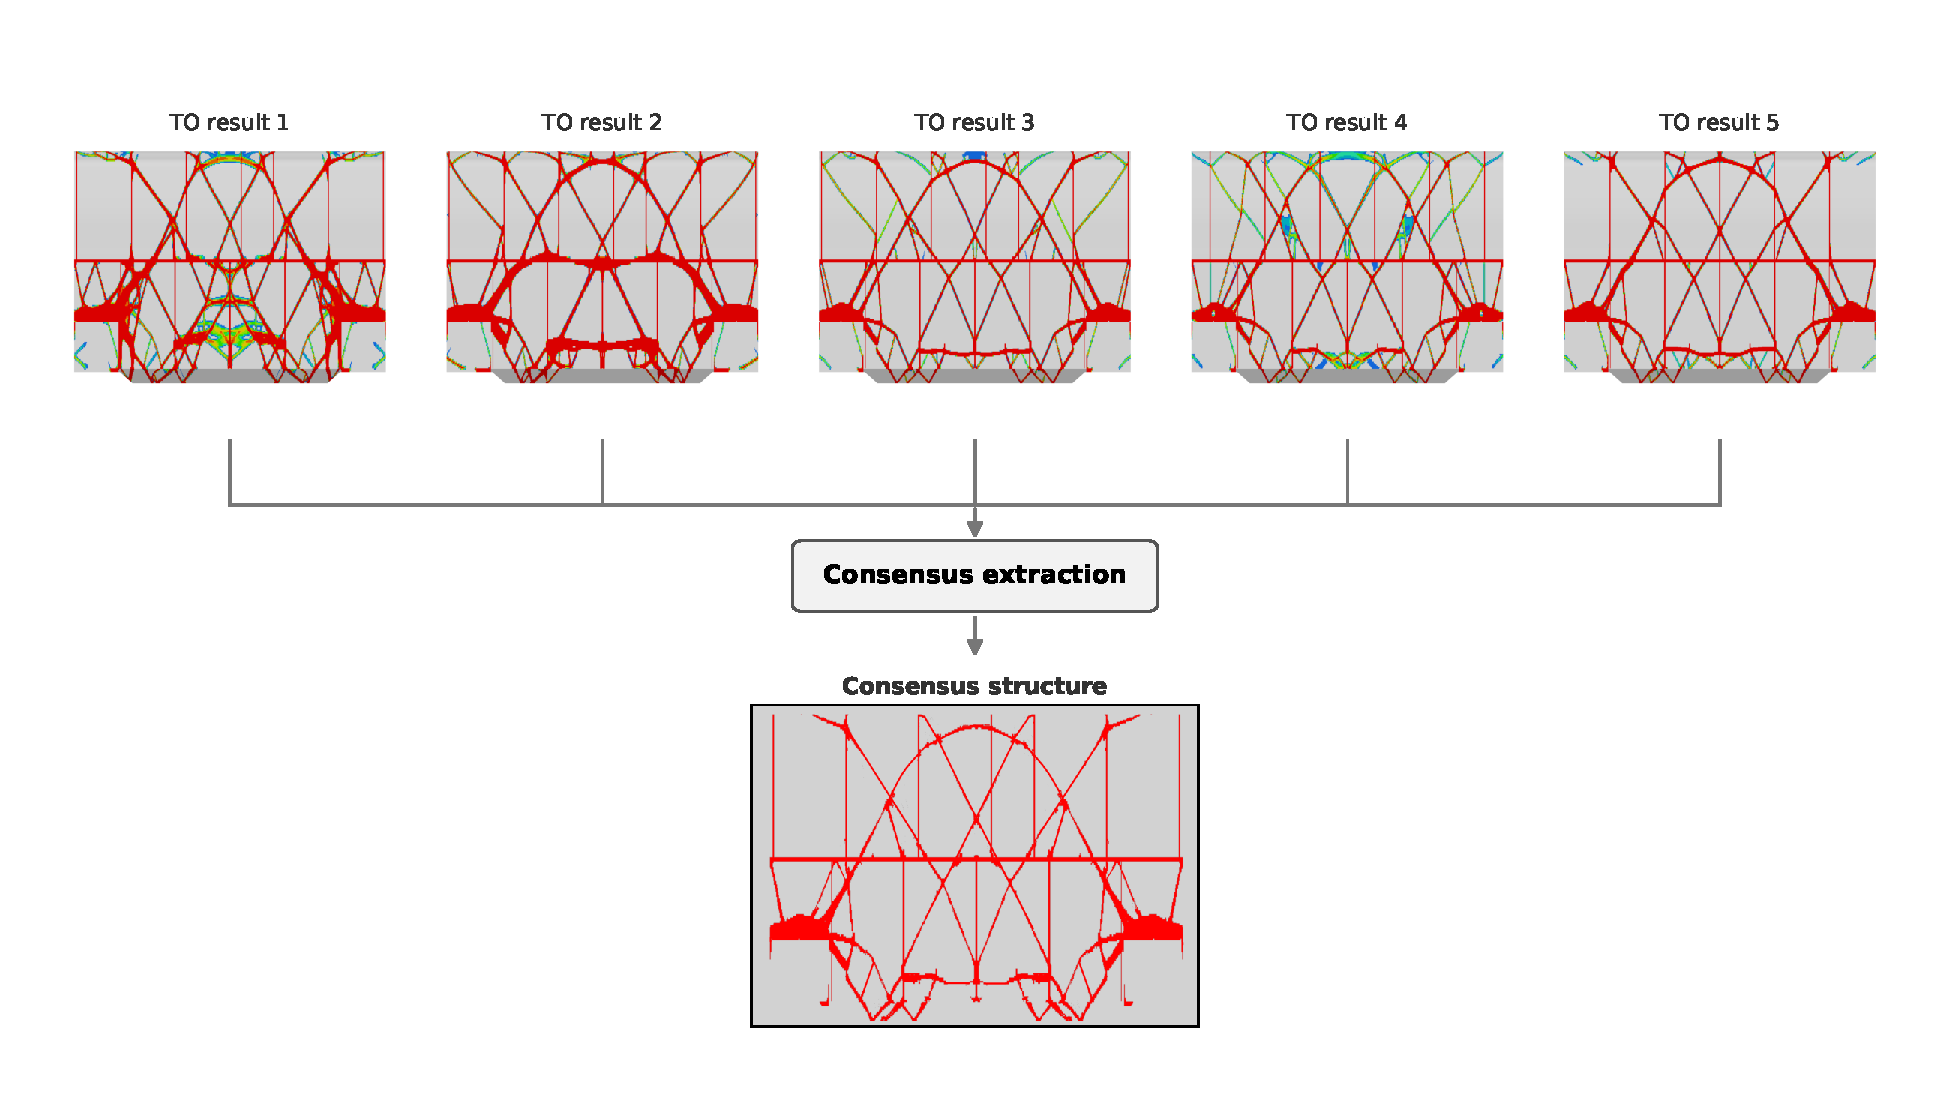
\includegraphics[width=0.8\textwidth]{consensus_figure.pdf}
	\caption{Problem Formulation : Extraction of common load paths from multiple TO results. The first row shows five different optimization results which are inputs and the bottom row presents the resulting consensus image representing the common load paths.}
	\label{fig:problemstat}
\end{figure}

The extracted consensus captures precisely these persistent dominant load paths, and its practical value lies in how it feeds back into the design loop. Rather than restarting each subsequent topology optimization from a uniform or blank design domain, the consensus provides an informed initialization that already encodes the robust, load-bearing skeleton common to all considered scenarios. In further optimization runs the consensus regions can be held fixed as solid material, so that the optimizer no longer needs to rediscover the dominant load paths and instead redistributes material only in the remaining free regions to satisfy case-specific requirements. This reduces the effective design space, promotes consistency across the resulting family of designs, and shortens convergence by sparing the repeated \gls{fea} iterations that would otherwise be spent
recovering the shared skeleton. In this way the consensus serves as a reusable, data-driven starting point that replaces the restarting from a blank design domain, offering a more systematic and reproducible route to a robust final design.

This interpretation task can be considered as a visual pattern recognition where the aim is identifying recurring geometric structure across a set of images. Understanding and modeling such visual patterns is a long standing problem in computer vision, and deep neural networks have become the common approach to it. Deep learning allows learning hierarchical representations directly from data rather than relying on hand crafted features. This motivates the central premise of this thesis: that the manual consensus finding step in topology optimization can be reformulated as a learnable pattern extraction problem and addressed with deep learning methods.The thesis aims to achieve its objectives by addressing the following key research questions:
\begin{itemize}
\item How can deep learning methods be effectively leveraged to identify and extract recurrent structural load paths from multiple \gls{to} results and, which network architectures are most suitable for this task?
\item How does the performance of deep learning based approaches compare with classical image processing methods such as pixel-wise averaging?
\end{itemize}

The thesis is organized as follows. First we give an overview about the problem and the basic background of both TO and deep learning in Chapter \ref{sec:background}. We discuss preliminary strategies from classical image processing approaches and other deep learning approaches addressing similar or problems closer to this idea in Chapter 3. Next we describe the proposed methodology  followed by the results and discussion in Chapter 4. Finally we present the summary and future outlook to improve the results in Chapter 5.



%%% ===============================================================================
\chapter{Background}\label{sec:background}
%%% ===============================================================================

% ---------------------------------------------------------------------------------
\section{Topology Optimization}\label{sec:background:topologyoptimization}
% ---------------------------------------------------------------------------------
The objective of \gls{to} is to identify the most efficient utilization of material while ensuring the structure meets specific physics-based performance requirements. A widely used approach is the \gls{simp} method \cite{c4}. The \gls{simp} method represents the material distribution through a continuous density field, where the density at each point indicates the proportion of material present in that region. The optimization proceeds by iteratively updating this density field to minimize an objective, subject to constraints such as a stress, deformation and prescribed material volume.In structural mechanics, a common objective is the minimum compliance problem, which seeks the material distribution that minimizes the deformation of the structure under prescribed loads and boundary conditions \cite{c5}.

Let $\Omega \subset \mathbb{R}^d$ represent a bounded design domain. A density field $\rho(x) \in [0, 1]$ describes how much material is present at each point $x$. $\rho = 0$ denotes void (no material) and $\rho = 1$ represents solid material.This density field is the design variable to be optimized. For a given material layout, the structure's response to the applied loads i.e, its displacement $u$ is obtained by solving the physical equilibrium equation $\mathbf{K}(\rho)\, u = f$, where $f$ is the load applied and
$\mathbf{K}(\rho)$ is the stiffness matrix determined by the material layout. The
TO problem is to find the density distribution $\rho$ that minimizes an objective function
$J$ typically the compliance (i.e.\ the inverse of stiffness) subject to the
equilibrium equation and a constraint on the maximum allowable material volume $V_{max}$. Figure \ref{fig:TOProcess} illustrates this overall TO process.
%
\begin{equation}
	\min_{\rho} \ J(\rho)
	\quad \text{s.t.} \quad
	\mathbf{K}(\rho)\, u = f,
	\qquad
	\int_{\Omega} \rho \, \mathrm{d}\mathbf{x} \leq V_{\max}.
	\label{eq:TO}
\end{equation}

\begin{figure}[htbp]
	\centering
	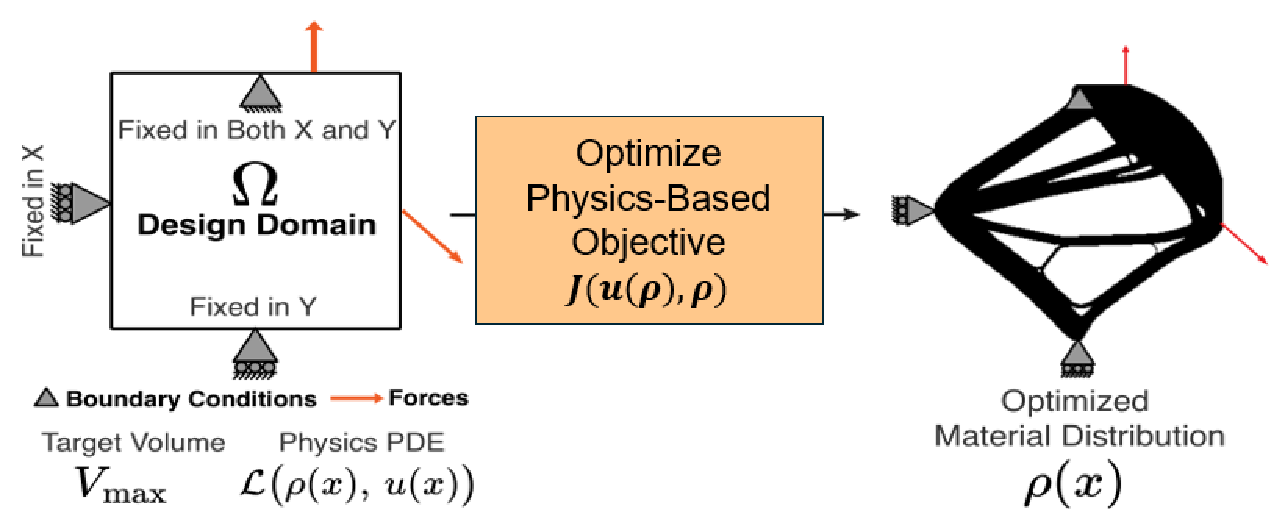
\includegraphics[width=0.8\textwidth]{TO Process.pdf}
	\caption{Overall TO process. The goal is to find a density field $\rho(x)$ to satisfy the objective function based on the given boundary conditions and applied forces \cite{c5}.}
	\label{fig:TOProcess}
\end{figure}

This problem doesn't have a closed form solution, so it is solved numerically. The domain $\Omega$ is divided into a mesh of finite elements, each with its own density value, and the equilibrium equation is solved by \gls{fea} at every iteration to evaluate the current design. Optimizer then updates the densities and repeats until convergence. Intuitively, the optimizer redistributes material according to how much each
region contributes to the overall stiffness, material is removed from lightly loaded regions, which carry fewer stress and contribute little to the structural performance, and reinforced along the primary load paths, where the stress is highest. Iterating this redistribution yields a structure in which material is concentrated where it is mechanically most effective.

While \gls{to} is most commonly applied to comparatively small components such as levers or brackets, in this work it is applied to large scale structures such as railway car bodies. Figure \ref{fig:to_result} shows a result of such an optimization. In general, the gray area is the design domain, within which material may be freely added or removed during optimization, whereas the white areas are non design regions, parts of the domain that are excluded from optimization, such as the openings for doors and windows. The colors encode element densities, red and orange indicate the higher density region and mark the primary load paths that form the structural backbone of the design, whereas green, blue corresponds to low density regions that carry relatively less load. 

\begin{figure}[htbp]
	\centering
	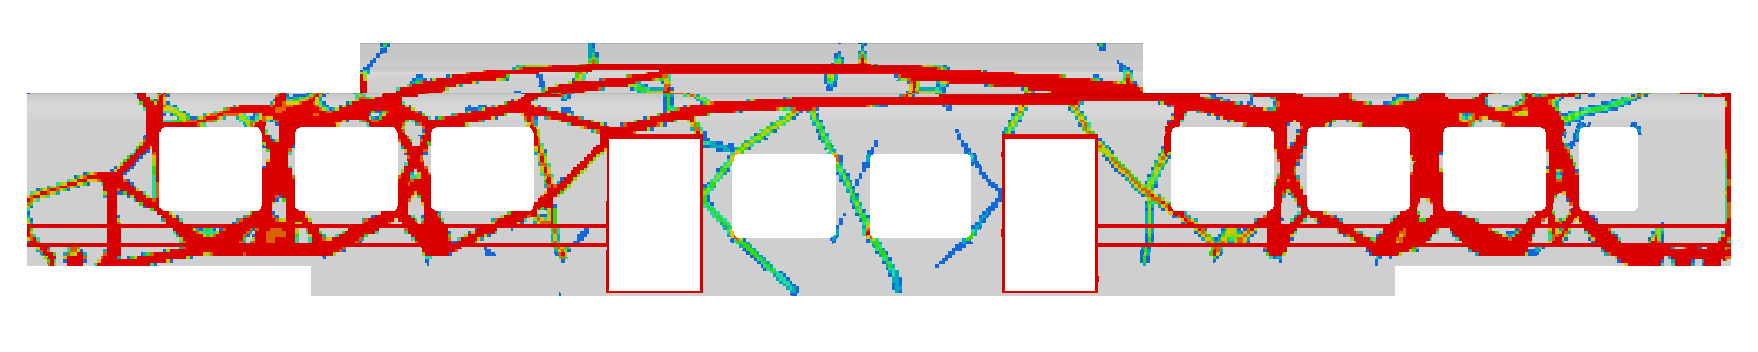
\includegraphics[width=0.8\textwidth, height=0.2\textheight]{TO_Result.pdf}
	\caption{Result of a TO on side wall of a railway car body. The gray region is the design domain, white areas are non-design regions, red indicates the main load paths and other colors represent relatively low material density regions.}
	\label{fig:to_result}
\end{figure}

The optimization is typically carried out on a three-dimensional (3D) model of the component. In this work, however, the resulting structures are represented and processed as two-dimensional (2D) images, which serve as the input to consensus extraction methods developed in the following chapters. Restricting the analysis to 2D keeps the problem tractable while retaining the essential information such as the spatial arrangement of load paths that the consensus task depends on.

% ---------------------------------------------------------------------------------
\section{Neural Networks}\label{sec:background:nn}
% ---------------------------------------------------------------------------------


% ---------------------------------------------------------------------------------
\subsection{Convolutional Neural Network}\label{sec:background:cnn}
% ---------------------------------------------------------------------------------
\gls{cnn} process image data by applying learned filters over local neighborhoods, sharing weights across spatial positions. This yields translation-equivariant feature extraction, with successive layers aggregating local patterns into increasingly large scale structure  \cite{c6}. \gls{cnn}s produce dense predictions at the resolution of input, making them directly applicable to image-to-image tasks such as consensus extraction, where both the input topology views and the output consensus are defined on the same pixel grid.
Rather than regressing the consensus directly, the network in this work adopts a residual formulation \cite{c7}. The pixelwise average of the input views from Section \ref{sec:pixelwiseavg} serves as a reference estimate, and the CNN predicts a correction that is added to it. This allows the model to start at a competitive baseline and focuses the learning to structured deviations such as thin members lost by averaging that the baseline fails to capture.

% ---------------------------------------------------------------------------------
\subsection{Variational Autoencoder}\label{sec:background:vae}
% ---------------------------------------------------------------------------------
\gls{vae} \cite{c8} shares the encoder-decoder structure of a traditional \gls{ae} \cite{c9}, but its mathematical foundation is quite different. Standard AE maps each input to a single fixed latent code, while a \gls{vae} encodes each input as a probability distribution over the latent space and is derived from a probabilistic generative model of the data.

The key idea behind the \gls{vae} is that every data point $x$ (images in our case) is generated from two steps: 
\begin{enumerate}
	\item a latent code $z$ is drawn from a prior distribution, typically a
	standard Gaussian, $z \sim p(z) = \mathcal{N}(0, I)$
	\item a neural network, the decoder that maps this code to a data point
	through a conditional distribution $p_\theta(x \mid z)$, where $\theta$ denotes
	the decoder parameters.
\end{enumerate}

The parameters $\theta$ should be chosen so as to maximize the probability assigned by the model to observed data. The likelihood of a single data point is obtained by marginalizing over all latent codes that could have produced it,
%
\begin{equation}
	p_\theta(x) = \int p_\theta(x \mid z)\, p(z)\, \mathrm{d}z .
	\label{eq:marginal}
\end{equation}
%
The computation of this integral is intractable as $z$ is high dimensional and continuous, so summing over every possible code is computationally infeasible. The same problem makes the true posterior $p_\theta(z \mid x)$ intractable, because by Bayes' rule it contains $p_\theta(x)$ in its denominator.

\paragraph{\textbf{Variational Approximation}}
\gls{vae} learns the approximation of this intractable posterior through a second network called the encoder $q_\phi(z \mid x)$ with parameters $\phi$. This network takes an input image and outputs the parameters, mean $\mu$ and a variance $\sigma^2$  of a Gaussian distribution for every latent dimension. Rather than searching the entire latent space for codes that explain $x$, we simply query the encoder for a good estimate. Figure \ref{fig:vae_arch} illustrates a typical \gls{vae} architecture.

\begin{figure}[htbp]
	\centering
	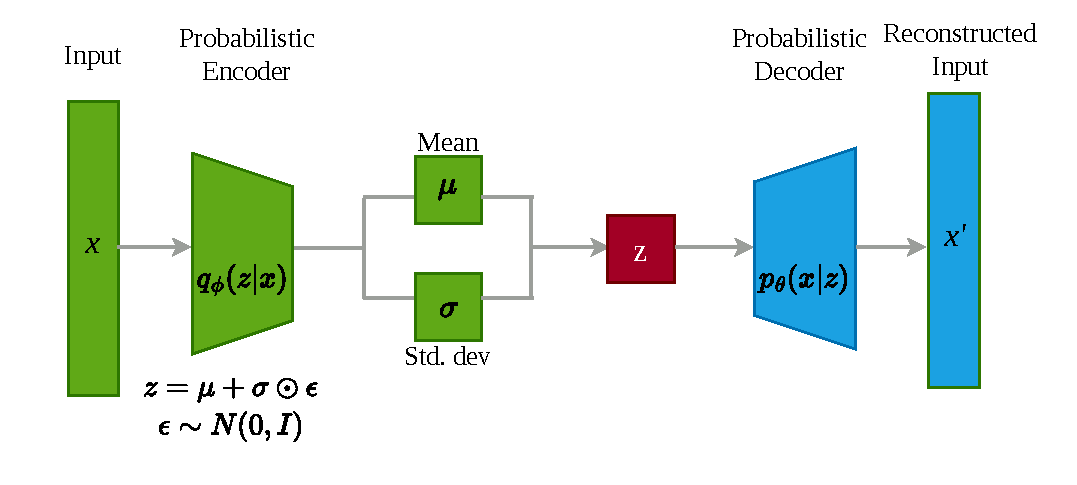
\includegraphics[width=0.8\textwidth]{VAE Architecture.pdf}
	\caption{Architecture of a VAE, consisting of an encoder that maps the input $x$ to a latent representation $z$ and a decoder that reconstructs the input $x'$ from the sampled latent variables \cite{c10}.}
	\label{fig:vae_arch}
\end{figure}

This approximation $q_\phi(z \mid x)$ must be close to true posterior $p_\theta(z \mid x)$ and the distance between two distributions can be measured with \gls{kl} divergence. $D_{\mathrm{KL}} (X\,\|\,Y)$ measures how much information is lost if distribution Y is used to represent X. We therefore have to find the $\phi$ that minimizes $D_{\mathrm{KL}}\!\left(q_\phi(z \mid x)\,\|\,
p_\theta(z \mid x)\right)$.

\paragraph{\textbf{\gls{elbo}}}
This KL term cannot be minimized directly, because it again involves the intractable posterior. However, starting from the log likelihood of the data one can show based on \cite{c10},
%
\begin{equation}
	\log p_\theta(x) =
	\underbrace{\mathbb{E}_{q_\phi(z \mid x)}\!\left[\log p_\theta(x \mid z)\right]
		- D_{\mathrm{KL}}\!\left(q_\phi(z \mid x)\,\|\,p(z)\right)}_{\displaystyle \mathcal{L}(\theta, \phi;\, x)\ \text{(ELBO)}}
	\; + \; D_{\mathrm{KL}}\!\left(q_\phi(z \mid x)\,\|\,p_\theta(z \mid x)\right).
	\label{eq:elbo_decomp}
\end{equation}
%
Because the KL divergence is non negative, the term $\mathcal{L}(\theta, \phi; x)$ is a lower bound on $\log p_\theta(x)$ and is known as the \gls{elbo}. Since $\log p_\theta(x)$ is fixed for a given data point, maximizing the \gls{elbo} simultaneously increases the data likelihood and drives the encoder $q_\phi(z \mid x)$ towards true posterior. Training a \gls{vae} therefore amounts to maximizing the \gls{elbo} jointly over $\theta$ and $\phi$.

The \gls{elbo} has an intuitive interpretation. Its first term, $\mathbb{E}_{q_\phi(z \mid x)}[\log p_\theta(x \mid z)]$, is a reconstruction term, it is large when codes sampled from the encoder allow the decoder to
reconstruct the input well. The second term, $D_{\mathrm{KL}}(q_\phi(z \mid x)\,\|\,p(z))$, is a regularization term that keeps the encoder's distribution close to the prior. For a Gaussian encoder
$q_\phi(z \mid x) = \mathcal{N}(\mu, \sigma^2 I)$ and a standard Gaussian prior, this term has the closed form
%
\begin{equation}
	D_{\mathrm{KL}}\!\left(q_\phi(z \mid x)\,\|\,p(z)\right)
	= -\tfrac{1}{2} \sum_{j=1}^{d}
	\left(1 + \log \sigma_j^2 - \mu_j^2 - \sigma_j^2\right),
	\label{eq:kl_gaussian}
\end{equation}
%
where $d$ is the dimensionality of the latent space, so it can be evaluated
directly during training.

\paragraph{\textbf{Reparameterization trick}}
One practical problem remains, the reconstruction term requires sampling $z$ from the encoder distribution, and sampling is a stochastic operation through which gradients cannot propagate back to $\phi$. The reparameterization trick \cite{c8} resolves this by moving the randomness out of the learnable path. Instead of sampling $z$ directly, we sample a noise variable $\epsilon \sim \mathcal{N}(0, I)$ that carries no learnable parameters, and then form the latent code deterministically as
%
\begin{equation}
	z = \mu + \sigma \odot \epsilon ,
	\label{eq:reparam}
\end{equation}
%
where $\odot$ denotes element wise multiplication. The randomness now enters only through $\epsilon$, so gradients can flow through $\mu$ and $\sigma$, and the whole model can be trained end-to-end with standard back propagation. In this work, input is a set of \gls{to} results \{$x_1,x_2,..,x_n$\} and each image is passed through a shared encoder $q_\phi(z \mid x_{i})$, which maps the image to a latent probability distribution characterized by its latent parameters. These representations are aggregated in the latent space to capture the common structural features shared across the input set. A latent code $z$ representing the consensus structure is sampled and decoded using $p_\theta(x' \mid z)$ to reconstruct the expected output structure $x'$.


%%% ===============================================================================
\chapter{Related Work}\label{sec:relatedwork}
%%% ===============================================================================

% ---------------------------------------------------------------------------------
\section{Deep Learning and Topology Optimization}\label{sec:relatedwork:dpandto}
% ---------------------------------------------------------------------------------

In recent years, \gls{dl} has been increasingly integrated into the \gls{to} pipeline to improve its efficiency and broaden its applicability. Such methods have been applied at several stages of the process such as accelerating the iterative optimization itself, building surrogate models that predict structural responses without repeated finite element analysis and even replacing the optimizer entirely with generative models that produce optimized designs directly \cite{c21}. A smaller body of work addresses the post processing and interpretation of \gls{to} results, which is where this thesis is situated. In the following, we review representative works in each of these directions and identify the research gap that motivates our approach.

\subsection{Acceleration of \gls{to} process}

A key limitation of \gls{to} is its high computational cost to generate optimized structures. As the mesh resolution increases the optimization process may take hours to days. Several studies have therefore aimed at accelerating the process. The first to incorporate a neural network into the \gls{to} loop was~\cite{c2}, who observed that the broad layout of the final structure emerges early in the optimization, while later iterations
mostly refine details. They exploit this by running only the first few iterations of the conventional optimizer and training a CNN to predict the final optimized topology directly from these intermediate results.

Figure~\ref{fig:TOML_1} illustrates the architecture with a encoder, decoder network and a final pixel wise classification layer. This approach reduced the total computation time by roughly a factor of twenty, and was later extended to three dimensions and to varying boundary and load conditions by \cite{c12}. \cite{c13} used deep belief network to predict the near optimal element density from the intermediate results and were further refined by \gls{simp} method.

\begin{figure}[htbp]
	\centering
	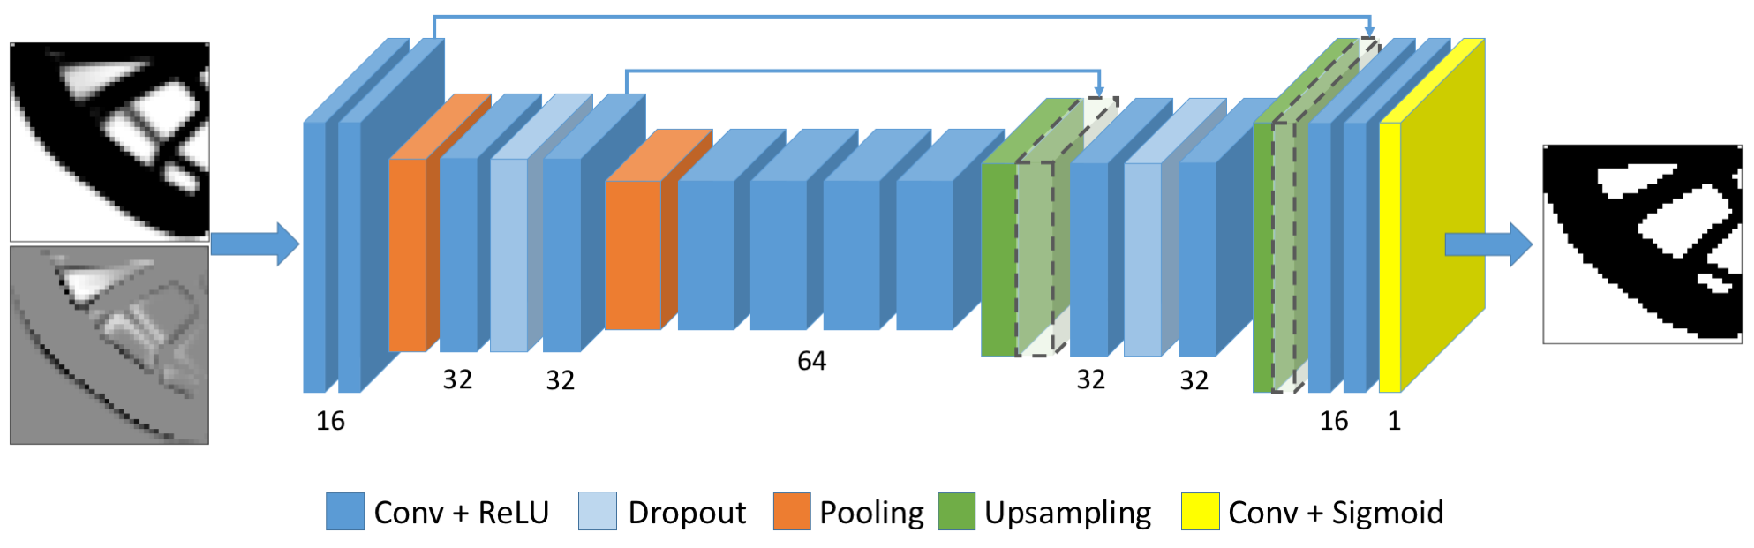
\includegraphics[width=0.8\textwidth]{TOML_1.pdf}
	\caption{\gls{cnn} architecture for obtaining optimal \gls{to} results from intermediate optimization results \cite{c2}.}
	\label{fig:TOML_1}
\end{figure}


\subsection{Generative Design}

Since the optimization process itself is expensive, another line of work replaces it with generative models that produce candidate designs directly, helping engineers explore diverse solutions for a given problem without running the full optimizer. Rawat and Shen \cite{c14} used a \gls{cwgan} to generate designs in a non iterative manner. Malviya et al.\cite{c15} studied the effectiveness of \gls{cnn}, UNet and \gls{gan} in generating designs under varying design constraints, loads, and boundary conditions. The study concluded TOPCNN and TOPGAN to be best performing models.

Of particular relevance to this thesis is a parallel line of work built on \gls{vae}, which demonstrates that topology optimized structures can be embedded in compact, structured latent spaces. Working with optimized heat conduction topologies, \cite{c16} study performs design exploration and optimization directly in a learned \gls{vae} latent space. A related approach attaches a stiffness regressor to a \gls{vae} so that the latent space explicitly encodes mechanical properties \cite{c17}. Figure \ref{fig:TOML_2} shows the \gls{vae} architecture whose decoder generates representative micro structures from the latent code. Rather than learning the latent space once, another method iteratively retrains a \gls{vae} on high-performing designs to converge toward optimal material distributions \cite{c18}. Beyond static designs, entire optimization trajectories have also been compressed into and predicted within a \gls{vae} latent space \cite{c19}. Collectively, these results establish an empirical premise that this thesis builds on that the latent representations of \gls{to} structures are smooth and semantically organized enough to support search, regression, and trajectory modeling. This further strengthen the claims that latent space operations such as interpolation, search and aggregation are meaningful.


\begin{figure}[htbp]
	\centering
	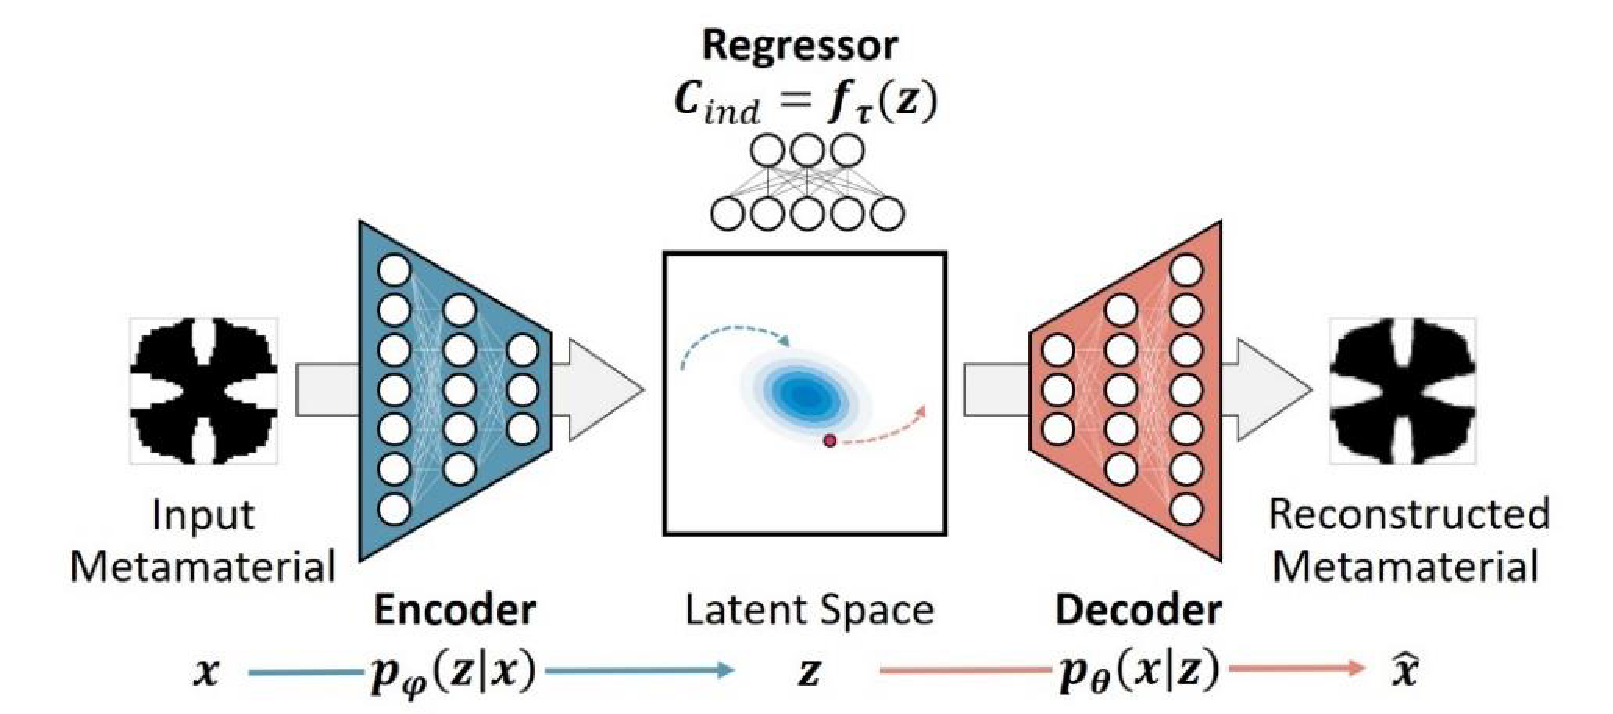
\includegraphics[width=0.8\textwidth]{TOML_2.pdf}
	\caption{Architecture of the \gls{vae} model with a stiffness regressor in the latent space used in representation and management of micro structures for multi-scale design \cite{c17}. }
	\label{fig:TOML_2}
\end{figure}

Models discussed so far are used to produce solutions and the resulting candidates are handed to a engineers for interpretation.However, the automated identification of the most relevant structural patterns among multiple generated solutions remains an open research gap that this thesis addresses.

The closest precursor to the approach developed in this thesis is the work of Ulu et al. \cite{c20}, who embed a set of optimized topologies into a linear latent space via \gls{pca}. A neural network is trained to map loading configurations to latent coefficients, synthesizing new optimal structures by decoding the predicted linear combination of eigen images. This work establishes, well before the deep generative literature, the core template of operating on existing \gls{to} solutions through latent space arithmetic. Its limitations, delineate exactly the requirements of this thesis, the linear \gls{pca} basis cannot guarantee that decoded combinations form connected, valid structures and gray superpositions must be resolved by thresholding. The formulation is deterministic, offering no representation of agreement between solutions and the task is interpolation across loading configurations rather than fusion of competing solutions to the same problem. This thesis uses a similar premise where the linear \gls{pca} basis is replaced with a nonlinear, probabilistic \gls{vae} manifold with connectivity aware supervision. Furthermore, our method is not conditioned on a load configuration, rather than predicting a design from prescribed loads, we aggregate multiple optimized solutions in the latent space.


% ---------------------------------------------------------------------------------
\section{Set Operations and Aggregation Methods}\label{sec:relatedwork:dpandto}
% ---------------------------------------------------------------------------------

The model developed in this thesis must accept a set of input images and map them to a single representative output image. Therefore, the methods reviewed below taken in multiple inputs and process them into a single output. These methods differ in the how multiple inputs are learned together from data and in the ultimate objectives some are combined representation, some are fusion, some are aggregation of views and some are disentanglement. 

The simplest learned method is the multi-view \gls{cnn}~\cite{c22}, which represents a 3D shapes as 2D images rendered from independent views and aggregates the multi-view information for shape recognition. Each image passes through a shared convolutional network, the resulting features are combined by element-wise max pooling, and a second network stage produces the shape descriptor. This study demonstrates that an unordered set of views can be combined to a single shape descriptor through pooling operation that improves the downstream recognition performance. %Add some literature with multi input residual cnn and good hook to start vae%

Multimodal \gls{vae} literature addresses the question of how to combine several input posteriors over a shared latent space into a single joint posterior. Wu and Goodman~\cite{c23} adopt product-of-experts(PoE) to approximate the joint posterior where the individual Gaussians are multiplied, which in closed form yields a combined precision equal to the sum of the individual precisions and a combined mean equal to the precision weighted average of the individual means.
%
\begin{equation}
	q(z \mid x_1, \dots, x_N) \;\propto\; p(z) \prod_{i=1}^{N} q_\phi(z \mid x_i),
	\qquad
	\sigma_{\text{PoE}}^{2} = \Big(\sum_{i=1}^{N}\sigma_i^{-2}\Big)^{-1},
	\qquad
	\mu_{\text{PoE}} = \sigma_{\text{PoE}}^{2}\sum_{i=1}^{N}\sigma_i^{-2}\mu_i ,
	\label{eq:poe}
\end{equation}
%
 The product acts as an intersection of beliefs each expert can veto regions of the latent space and the joint becomes sharper with every additional input. In~\cite{c23} $N$ inputs are heterogeneous modalities of a single
 entity and the joint latent is decoded back into every modality. However, in this thesis the inputs are homogeneous $N$  \gls{to} results of the same type, encoded by a shared encoder and decoded into a single consensus output. We use the combination rule of Eq.~\eqref{eq:poe} as one of out aggreagtion method in our ablation studies. Mixture-of-experts Multimodal Variational Autoencoder (MMVAE) ~\cite{c24} replaces the product with a mixture-of-experts (MoE) posterior, a uniform mixture of the individual input Gaussians, motivated by the tendency of a single overconfident expert to dominate the PoE joint posterior. As a result, conflicting views survive as separate modes and no sharpening occurs, so disagreement is fully preserved but the formulation never commits to a single estimate, which a consensus task ultimately requires. Sampling from the mixture returns one view's explanation at a time, a candidate rather than a consensus. 
 
 %Two limitations are relevant. First, the formulation was subsequently criticised for producing generated outputs of adequate individual quality but weak coherence across modalities, which motivated the mixture-based alternative discussed below. Second, and more directly consequential here, the combined variance in Eq.~\eqref{eq:poe} depends only on the individual precisions and not on the separation of the individual means. Views that agree closely and views proposing entirely different structures therefore yield the same combined confidence, with the mean placed somewhere between them: disagreement is invisible to the joint uncertainty. This behaviour is appropriate when disagreement reflects observation noise around a single true value, but not when it reflects genuine ambiguity between equally valid designs. Add this in PoE abalation discussion study%

The method developed in this thesis is closely related to AttSets~\cite{c25}, which is designed to reconstruct a 3D shape from an arbitrary number of input views. The architecture consists of a encoder, decoder network with a  aggregation module in the latent space. Instead of a fixed pooling operator, the module in the latent space learns an score for each element of the deep feature set and aggregates by weighted summation and avoids the loss information due to mean and max pooling. The authors introduce a two stage training algorithm Feature-Attention Separate training (FASet), which first trains the base encoder-decoder on individual elements. In the second stage encoder-decoder is frozen entirely and only the parameters of attention module are optimized. The network generalizes to an arbitrary number of input images, a desirable property when consensus groups vary in size. %The aggregation weights in AttSets are produced by a learned scoring function applied to each feature and normalised across the set. They are therefore free parameters, constrained only to be non-negative and to sum to one, with no prescribed relationship to any property of the input.%


FusionVAE \cite{c27} is a hierarchical \gls{vae} that generates samples conditioned on multiple noisy, occluded or partially visible input images, optimizing a variational lower bound on the conditional log-likelihood. Each input is passed through a shared encoder, and the resulting context features are combined in the latent space rather than in image space. The fusion is applied hierarchically at every latent level, the per-input feature maps are aggregated pixel-wise using max operation into a single context feature map. The feature map produced by the generator at the preceding coarser level is added pixel-wise to the context feature map so that the fusion of the inputs at a fine scale is conditioned on the coarse scale reconstruction rather than performed independently at each resolution. In an ablation of the aggregation
operation, the authors report that max and mean aggregation outperform a Bayesian aggregation rule. This thesis also treats the aggregation operation as a design choice and compares the performance of mean, product of Gaussians and learned aggregation in the latent space.

Multi-level \gls{vae} \cite{c28} learns disentangled representations from grouped data where samples share a common attribute, such as identity or shape. The latent space is partitioned into content variable,
capturing the factor shared across a group and style variable, specific to each observation. The model learns to isolate shared group traits from individual variations. Contrastive \gls{vae}s pursue a related
decomposition, splitting the latent space into common and salient subspaces by means of separate encoders trained with dedicated loss terms. These methods~\cite{c30, c31}, are formulated for a background or target regime in which the salient content is a categorically distinct signal superimposed on a shared background. Our problem is quite different where the inputs share a common structure and differ only through small structural perturbations or functionally equivalent alternatives, so the variation to be separated is
of the same nature as the shared content rather than a distinct, superimposed factor.
 
Common to all of these architectures is the requirement that, since the inputs form a set and carry no meaningful ordering, the aggregation operator must be permutation invariant. This requirement was formalized by
Deep Sets~\cite{c29}, which characterizes permutation-invariant functions on sets as a per-element transformation $\phi$ applied to each member, followed by a symmetric aggregation such as summation, mean or max, and a subsequent nonlinear transformation $\rho$ of the aggregated representation. The architectures developed in this thesis follow the encode-aggregate-transform framework, which guarantees that the predicted
consensus is invariant to the order in which the input elements are presented.

Across all of the work discussed above have the inputs complementary such as different views, degraded observations, or modalities of a single underlying object. Here, aggregation serves to accumulate evidence and complete missing information. In the setting of this thesis, the inputs are competing where each candidate is a complete solution to the same optimization problem and aggregation must suppress substantive disagreement and recover a common underlying structure. To the best of our knowledge, no existing method specifically addresses the extraction of common structural patterns from collections of topology optimization results.


%%% ===============================================================================
\chapter{Preliminary Strategies}\label{sec:prelim_work}
%%% ===============================================================================


% ---------------------------------------------------------------------------------
\section{Pixel wise Averaging Method}\label{sec:pixelwiseavg}
% ---------------------------------------------------------------------------------

The most direct approach to consensus extraction operates in the pixel space of the images. Each image is represented on a common grid by a binarized density field $\rho_i(\mathbf{x})$ taking the value $0$ for void, $1$ for material. Given a group of $n$ inputs, the pixel-wise mean, $c(x) = \frac{1}{n} \sum_{i} \rho_{i}(x)$ assigns to every pixel the mean intensity across the group. The averaged result is not a discrete structural representation but a gray-scale agreement map where structures from individual inputs appear with varying levels of support. Values close to one identify regions where all solutions consistently contain material, values near zero are regions where all solutions contain void and intermediate values mark partial agreement. This method requires no training and introduces no learnable parameters beyond the group itself and remains invariant to ordering of the inputs. Therefore, it serves as a natural starting point and as the reference against which every learned method in this thesis are evaluated.

Since only the structures supported by a majority of the inputs are of interest, converting the agreement map into a consensus structure requires a threshold $t$. The pixels with value above $t$ are assigned to material and values below to void. Figure \ref{fig:supportcount} shows the super imposition of all the input images of a group, colored by the number of inputs that place material at each pixel. The lower region shown in red is supported by nearly all inputs where the structures overlap exactly. The diagonal members in the upper region behave differently. Although they are present in every solution, they are not spatially aligned, so their support is distributed over neighboring pixel locations and the count at any single location remains low.

\begin{figure}[htbp]
	\centering
		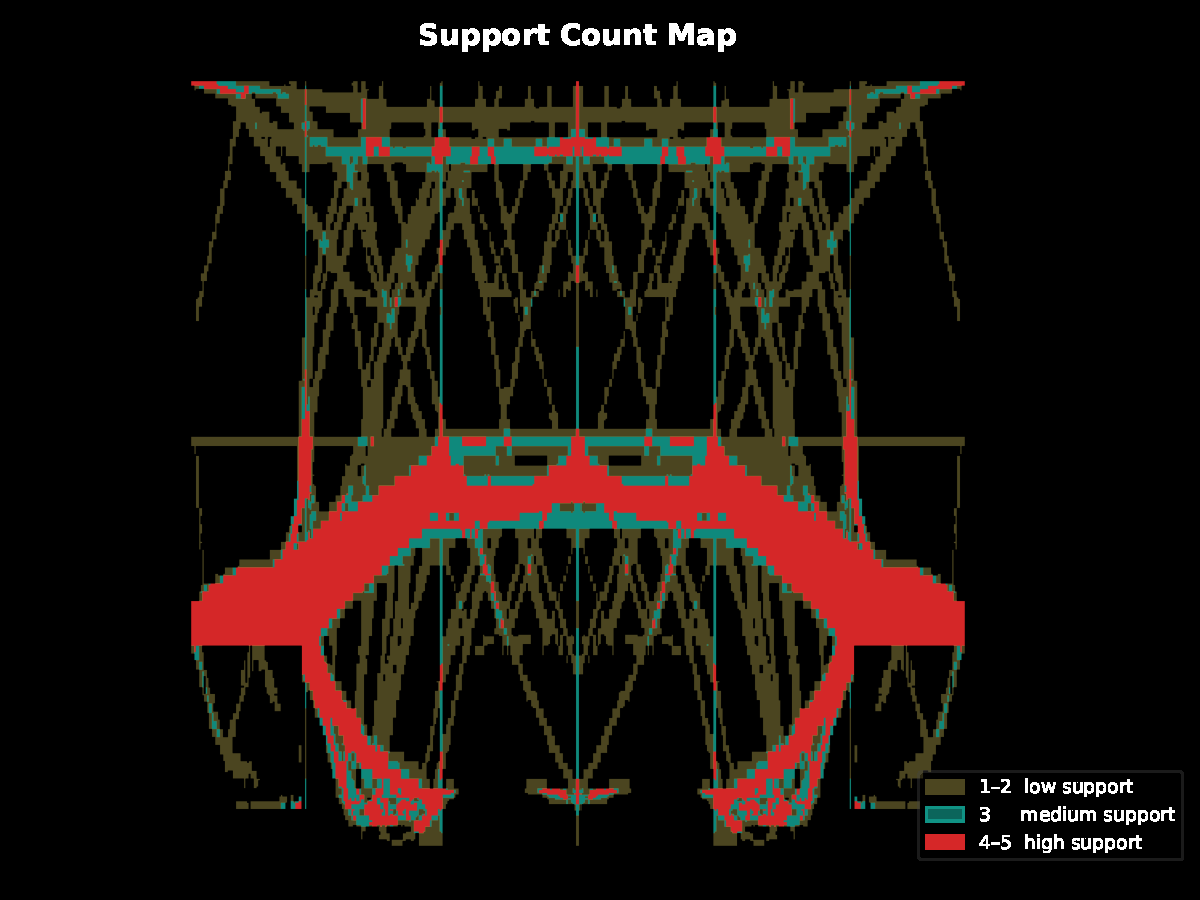
\includegraphics[width=0.4\textwidth]{Support Count.pdf}
	\caption{Super imposition of input images colored by the number of solutions that place material at each pixel. It also depicts the spatial misalignment in the inputs of similar structures.}
	\label{fig:supportcount}
\end{figure}


The choice of $t$ determines the outcome, which ranges from the union of all solutions at low thresholds to their near-intersection at high thresholds. A high threshold retains only strongly agreed-upon features, producing a sparse structure from which weakly supported members are removed while a low threshold retains weakly supported features, producing a dense structure in which mutually exclusive alternatives from different solutions appear simultaneously. To use this method as a baseline, a single threshold was fixed for all instances in the data. It was selected by sweeping $t$ across its range and, for each value, evaluating the resulting consensus structures against the reference targets using the \gls{cld} metric (more details in Section~\ref{cldice}). The value maximizing \gls{cld} was retained, yielding $t = 0.4$. Because this threshold is tuned directly against the reference targets, the baseline is given its best case single threshold performance a deliberately strong configuration, so that improvements reported over it are conservative.


\begin{figure}[htbp]
	\centering
	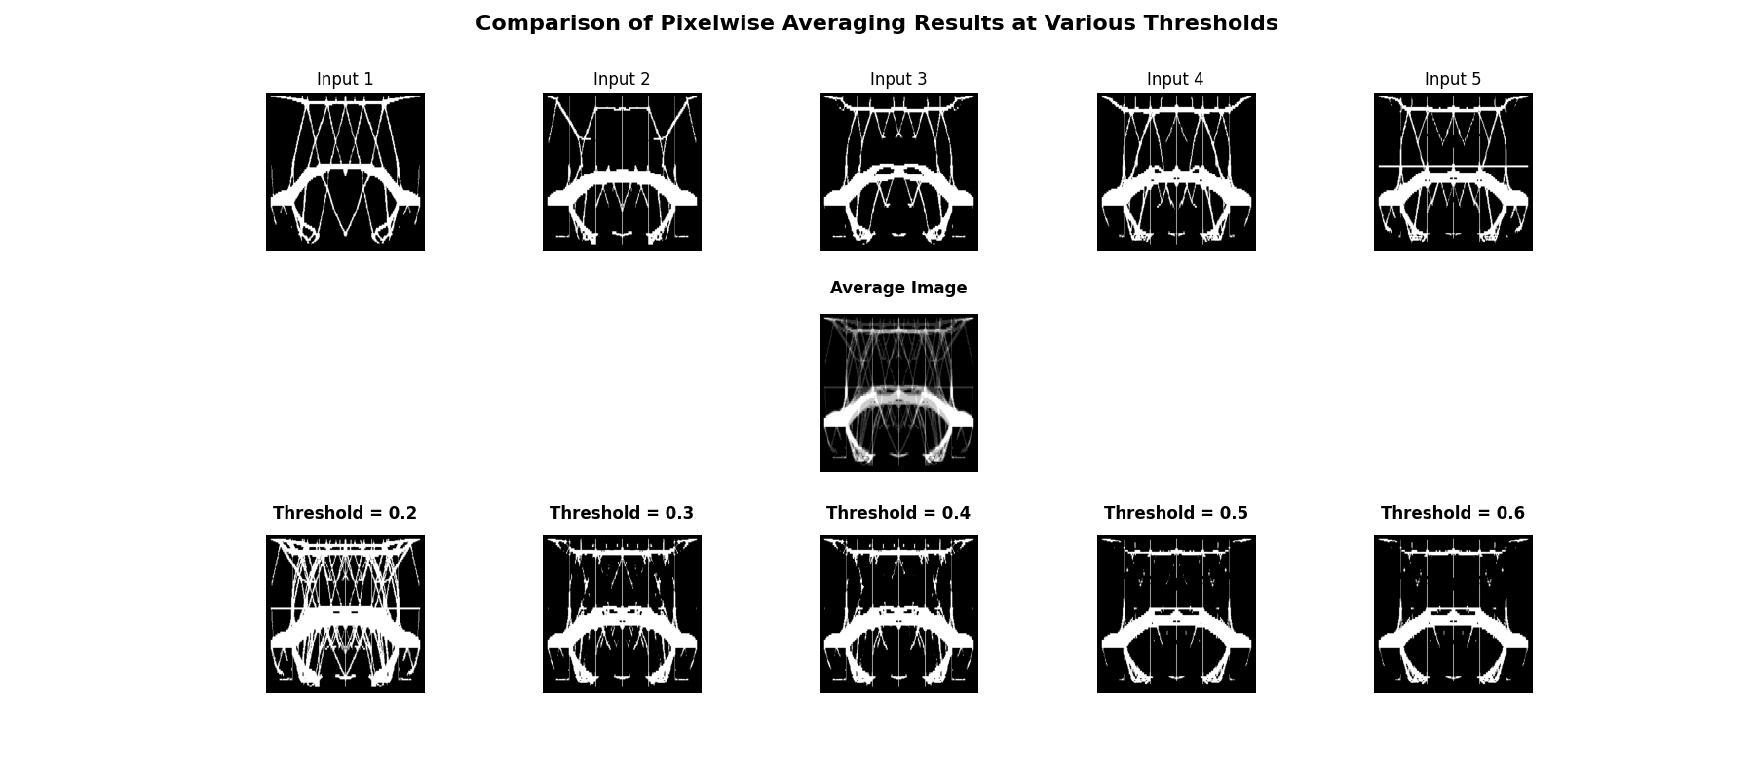
\includegraphics[width=0.9\textwidth]{Threshold_results1.pdf}
	\caption{Pixelwise averaging results at different thresholds. The top row represents the input images, center row represent the averaged result and the last row shows the results with various thresholds applied to the averaged result.}
	\label{fig:pixelwise_result}
\end{figure}

Thresholding is applied independently at each pixel and is therefore unaware of structural connectivity. As a result, a thresholded average may contain members that terminate without connecting to the remainder of the structure. Load paths are interrupted when averaged densities drop below $t$ resulting in disconnected fragments. Although morphological post-processing can remove small isolated regions and close minor gaps, it cannot recover load paths whose supporting evidence has been lost during the process. The information identifying which of several alternatives to retain is no longer present in the averaged field. Consequently, connectivity is not explicitly considered or controlled during the procedure instead, it emerges only as an indirect consequence of the selected threshold.


This thresholding step exposes the central weakness of pixel-space averaging, it assumes that corresponding structural features are spatially aligned across inputs. A structural member that is present in every solution but positioned slightly differently across inputs is smeared over several pixel locations, so its averaged density at any single location may never reach $t$ and the member is lost even though all solutions agree it should be present. This is evident from the Figure \ref{fig:pixelwise_result}, where the consensus structure obtained at threshold $t = 0.4$ does not include the diagonal members in the upper region. As illustrated in Figure \ref{fig:supportcount}, these structures receive insufficient pixel-wise support because their spatial positions vary between solutions. Furthermore, the resulting consensus contains disconnected segments and broken load paths, leading to structurally implausible representations. Pixel averaging thus conflates genuine structural disagreement with mere spatial misalignment of agreed-upon structure. This limitation motivates the development of aggregation methods in the following sections that can capture agreement beyond exact pixel correspondence.



% ---------------------------------------------------------------------------------
\section{Feature Based Methods}\label{sec:featurebased}
% ---------------------------------------------------------------------------------

The limitation of pixelwise aggregation described in Section \ref{sec:pixelwiseavg} arises from the assumption of exact spatial alignment between inputs. Structurally equivalent members may occupy different pixel positions across optimization results, causing operations defined on pixel coordinates to combine features that do not correspond. This observation suggests an alternate strategy, rather than aggregating at fixed pixel coordinates, correspondence between solutions can first be established, followed by aggregation of the corresponding structural features. Such a pipeline has two stages: a matching stage that identifies corresponding regions or features between solutions and an aggregation stage that forms a single consensus structure by combining the matched features. If reliable point-to-point correspondences existed between structurally equivalent members across inputs, consensus could in principle be formulated as a registration and voting problem, without any learned components. Therefore, the correspondence estimation stage was investigated first, as the success of any subsequent aggregation relies on the quality of the established matches.

We used the \gls{sift} \cite{c32}, a standard method for establishing sparse correspondences between images. SIFT detects keypoints as extrema in a difference-of-Gaussian scale space and describes the neighbourhood of each keypoint by a 128-dimensional histogram of local gradient orientations, normalised for dominant orientation and contrast. Correspondence is established by nearest-neighbour search in descriptor space, filtered by Lowe's ratio test, which discards a match when the distance to the closest descriptor is not sufficiently smaller than the distance to the second closest. This is an indication that the descriptor cannot discriminate between multiple candidate locations. Owing to its invariance to translation, rotation, and moderate scale changes, \gls{sift} is widely used for matching corresponding structures across images. Since the primary limitation of pixel-wise averaging arises from spatial misalignment of structurally equivalent members, \gls{sift} remedies it by establishing the correspondences required before aggregation.

To assess whether reliable correspondences could indeed be established, we applied SIFT to pairs of solutions from the same design problem. Approximately, 93\% of candidate matches were rejected by the ratio test. The detector itself performed as expected, returning keypoints along member boundaries and at junctions. The failure lies entirely in descriptor distinctiveness. \gls{to} outputs consist of thin members of nearly uniform width connected at junctions with highly repetitive local geometry. Consequently, a local neighbourhood around one keypoint is often indistinguishable from many others, giving rise to multiple equally plausible correspondence candidates. The ratio test therefore rejects most matches because no single descriptor is sufficiently more similar than the alternatives. Geometrically different configurations, such as V-shaped junctions with different opening angles, can fulfil the same mechanical function, while visually similar local patches may belong to entirely different structural members. Consequently, local image descriptors are insufficient to establish meaningful semantic correspondences in this domain.


\begin{figure}[htbp]
	\centering
	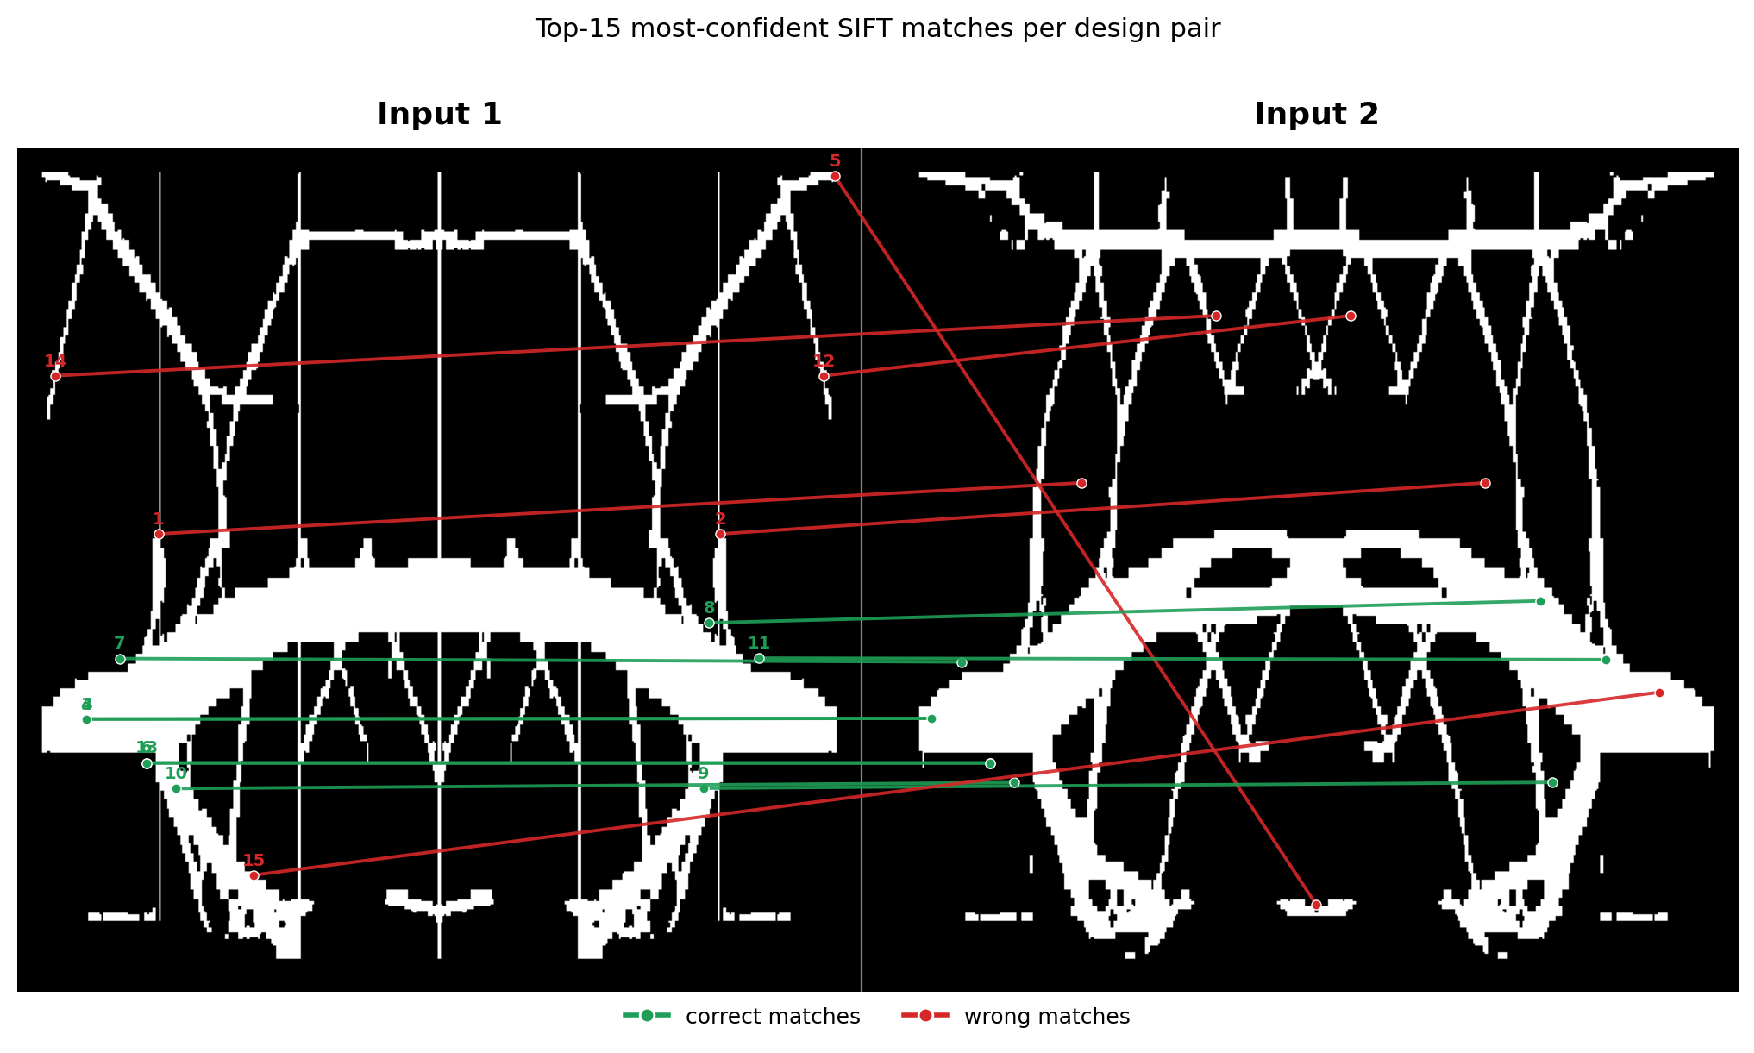
\includegraphics[width=0.7\textwidth]{sift_top10_matches.pdf}
	\caption{}
	\label{fig:siftres}
\end{figure}


Feature matching operates at the wrong granularity. It establishes correspondences between individual keypoints, whereas consensus must be formed over structural members. The relevant question is whether a member in one solution is the same structural feature as a member in another and answering it from point matches requires a grouping step that feature matching does not provide. 

The ambiguity that defeats SIFT at the descriptor level is the same phenomenon that later reappears at the structural level as the functional equivalence problem (Section X.X): Any method restricted to local evidence, whether hand-crafted descriptors or convolutional networks with limited receptive fields, faces the same fundamental limitation.
This finding shaped the direction of the thesis in two ways. First, it ruled out registration-based consensus pipelines, since no reliable dense correspondence could be established. Second, it motivated the move toward global latent representations, in which consensus is formed not by matching local features across views but by aggregating whole-structure encodings — the approach developed in Chapter X.
It motivates the approach developed in Chapter X, in which correspondence is not established explicitly at all: solutions are encoded into a learned representation and aggregated there, leaving a decoder trained on valid structures to produce a single consensus structure.


%%% ===============================================================================
\chapter{Methodology}\label{sec:method}
%%% ===============================================================================



% ---------------------------------------------------------------------------------
\section{Dataset Preparation}\label{sec:datasetprep}
% ---------------------------------------------------------------------------------




% ---------------------------------------------------------------------------------
\section{Residual Convolutional Neural Network}\label{sec:rcnn}
% ---------------------------------------------------------------------------------

% ---------------------------------------------------------------------------------
\section{Variational Autoencoder}\label{sec:rcnn}
% ---------------------------------------------------------------------------------


%%% ===============================================================================
\chapter{Results \& Discussion}\label{sec:method}
%%% ===============================================================================

This section presents the experimental evaluation of the proposed residual \gls{cnn} described in Section~\ref{sec:rcnn} for consensus extraction  of topology-optimized structures. The objective of this evaluation is to determine whether the proposed method can identify recurring load paths across multiple topology optimization solutions while preserving structural connectivity. The proposed approach is compared against the pixel-wise averaging baseline introduced in Section~\ref{sec:pixelwiseavg}.

The evaluation is performed using the metrics described in Section~\ref{metrics}, including the connectivity-aware \gls{cld} metric, its precision and recall components. While conventional pixel-wise metrics measure overlap between predicted and reference structures, clDice additionally evaluates the preservation of topological connectivity, which is particularly important for load-path extraction.

Figure~\ref{fig:rcnn_res1} shows 


\begin{figure}[htbp]
	\centering
	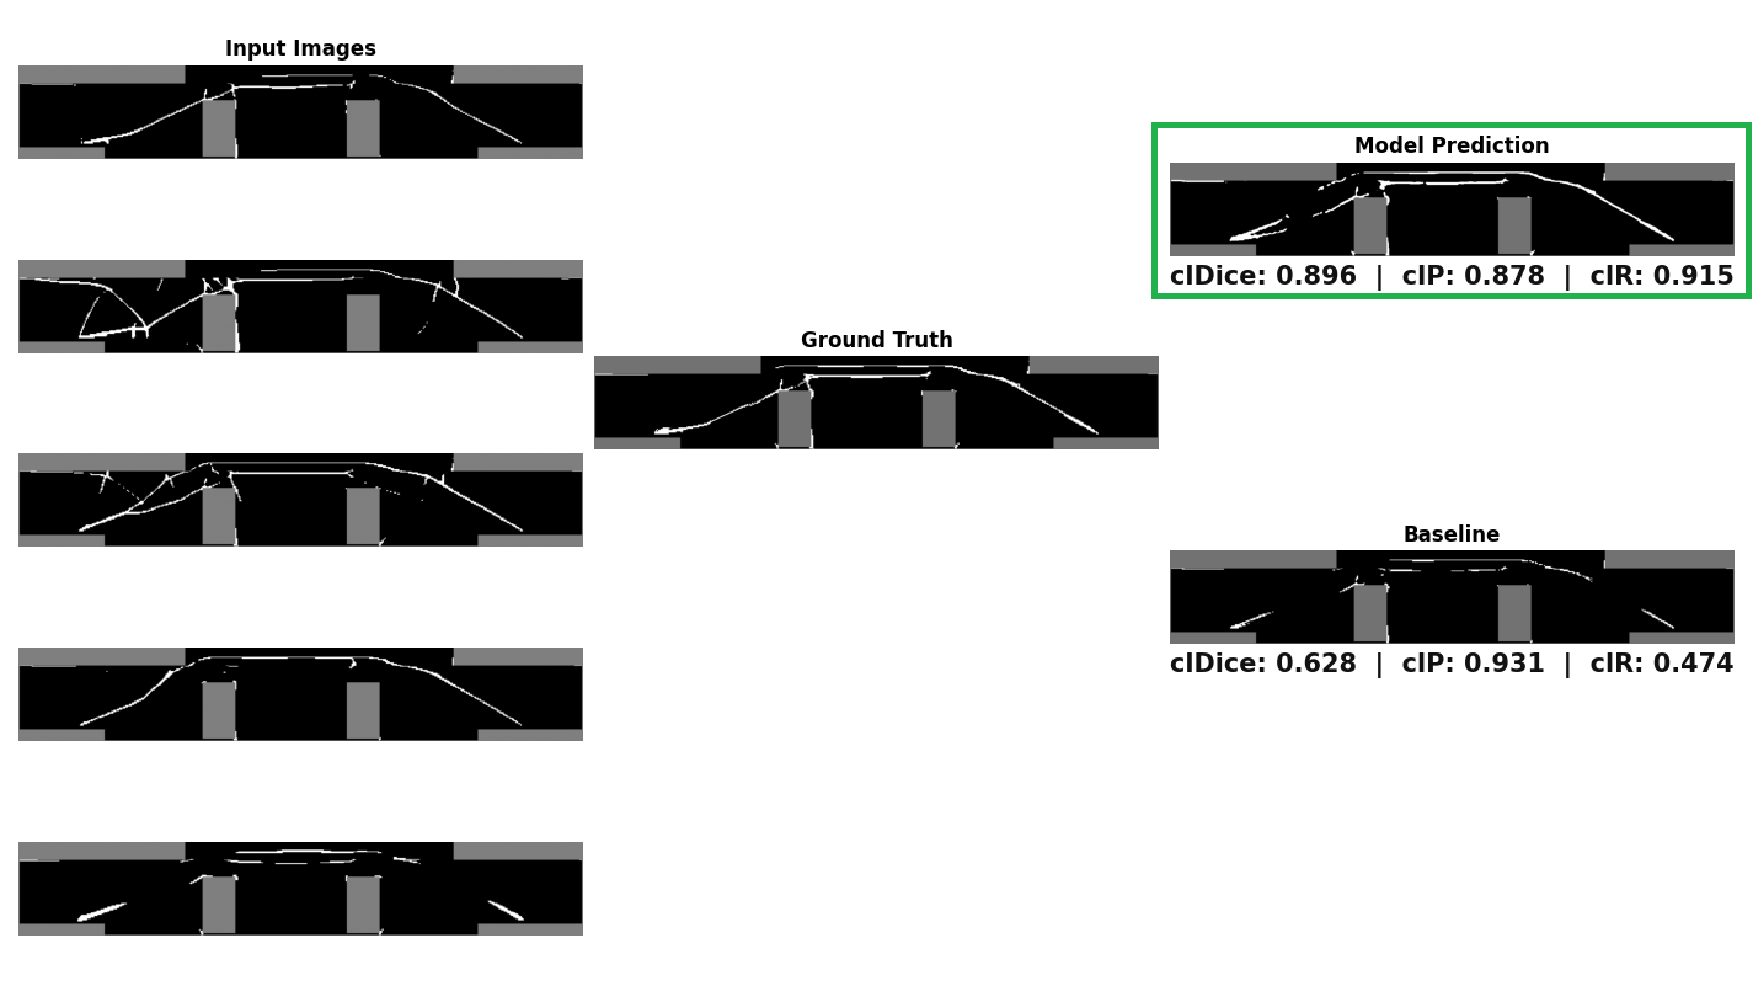
\includegraphics[width=0.9\textwidth]{CNN_Results1.pdf}
	\caption{}
	\label{fig:rcnn_res1}
\end{figure}




%%% ===============================================================================
%%% Bibliography
%%% ===============================================================================

\printbibliography

% Enfore empty line after bibliography
\ \\
%
\noindent
All links were last followed on July 28, 2026.

%%% ===============================================================================

%\IfDefined{printindex}{\printindex}
%\IfDefined{printnomenclature}{\printnomenclature}

\clearpage
\appendix
% 'Anhang' ins Inhaltsverzeichnis
%\phantomsection
%\addcontentsline{toc}{chapter}{Appendix}
\addcontentsline{toc}{part}{Appendix}

%%% ===============================================================================
\chapter{My first appendix}\label{sec:appendix1}
%%% ===============================================================================

\lipsum[1]

\pagestyle{empty}
\renewcommand*{\chapterpagestyle}{empty}
\Versicherung
\end{document}
